%\documentclass[review,3p]{elsarticle}
%\documentclass[preprint,3p]{elsarticle}
\documentclass[3p]{elsarticle}

%\usepackage{lineno,hyperref}
%\modulolinenumbers[5]

\journal{Information Science}
\usepackage[spanish]{babel}
\selectlanguage{spanish}
\usepackage[utf8]{inputenc}
\usepackage{graphicx}
%\usepackage{cite}
\usepackage{amsmath}
\usepackage{mathtools}
\usepackage{multirow}
%\usepackage{algpseudocode}
%\usepackage[none]{hyphenat}
\usepackage{algorithm}
\usepackage{hyperref}
\usepackage[noend]{algorithmic}
%\usepackage[]{algorithm2e}
\usepackage[normalem]{ulem}
 \useunder{\uline}{\ul}{}


\newcommand{\DCN}{{\sc dcn}}
\newcommand{\DE}{{\sc de}}
\newcommand{\DEEDM}{{\sc de-edm}}
\newcommand{\EAS}{{\sc ea}s}
\newcommand{\EA}{{\sc ea}}
\newcommand{\RMDDC}{{\sc rmddc}}
\newcommand{\CEC}{{\sc cec}}
\newcommand{\DSBX}{{\sc dsbx}}
\newcommand{\SBX}{{\sc sbx}}
\newcommand{\BLX}{{\sc blx}}
\newcommand{\UNDX}{{\sc undx}}
\newcommand{\SPX}{{\sc spx}}
\newcommand{\MOEAS}{{\sc moea}s}
\newcommand{\MOEA}{{\sc moea}}
\newcommand{\SMSEMOA}{{\sc SMS-EMOA}}
\newcommand{\MOP}{{\sc MOP}}
\newcommand{\MOEAD}{{\sc MOEA/D}}
\newcommand{\MOEADDE}{{\sc MOEA/D-DE}}
\newcommand{\NSGAII}{{\sc NSGA-II}}
\newcommand{\DEMO}{{\sc demo}}
\newcommand{\WFG}{{\sc wfg}}
\newcommand{\DTLZ}{{\sc dtlz}}
\newcommand{\UF}{{\sc uf}}
%


%%%%%%%%%%%%%%%%%%%%%%%
%% Elsevier bibliography styles
%%%%%%%%%%%%%%%%%%%%%%%
%% To change the style, put a % in front of the second line of the current style and
%% remove the % from the second line of the style you would like to use.
%%%%%%%%%%%%%%%%%%%%%%%

%% Numbered
%\bibliographystyle{model1-num-names}

%% Numbered without titles
%\bibliographystyle{model1a-num-names}

%% Harvard
%\bibliographystyle{model2-names.bst}\biboptions{authoryear}

%% Vancouver numbered
%\usepackage{numcompress}\bibliographystyle{model3-num-names}

%% Vancouver name/year
%\usepackage{numcompress}\bibliographystyle{model4-names}\biboptions{authoryear}

%% APA style
%\bibliographystyle{model5-names}\biboptions{authoryear}

%% AMA style
%\usepackage{numcompress}\bibliographystyle{model6-num-names}
\usepackage{xcolor}
%% `Elsevier LaTeX' style
\bibliographystyle{elsart-num-sort}
%%%%%%%%%%%%%%%%%%%%%%%

%\newcommand{\EAS}{{\sc ea}s}
%\newcommand{\CDE}{c{\sc de}}
%\newcommand{\DE}{{\sc de}}
%\newcommand{\HMR}{{\sc hmr}}
%\newcommand{\METCO}{\mbox{\sc{metco}}{}}
%\newcommand{\NP}{{\sc np}}

\renewcommand\spanishtablename{Tabla}
\begin{document}

\begin{frontmatter}

\title{Importancia de la Diversidad en el Diseño de Algoritmos Evolutivos}
%\tnotetext[mytitlenote]{Fully documented templates are available in the elsarticle package on \href{http://www.ctan.org/tex-archive/macros/latex/contrib/elsarticle}{CTAN}.}

%% or include affiliations in footnotes:
\author[label1]{Carlos Segura\corref{cor1}}
\ead{carlos.segura@cimat.mx}

\author[label1]{Joel Chac\'on Castillo}
\ead{joel.chacon@cimat.mx}


%\cortext[cor1]{Corresponding author. Tel.: + 52 473 732 7155}
\cortext[cor1]{Correspondiente al autor. Tel.: + 52 473 732 7155}
\address[label1]{Área de Ciencias de la Computación, Centro de Investigación de Matemáticas (CIMAT), Callej\'on Jalisco s/n, Mineral de Valenciana, Guanajuato, Guanajuato 36240, Mexico}
%\address[label1]{Area of Computer Science, Centre for Research in Mathematics (CIMAT), Callej\'on Jalisco s/n, Mineral de Valenciana, Guanajuato, Guanajuato 36240, Mexico}

\begin{abstract}
La convergencia prematura es una de las mayores desventajas que afectan el rendimiento de los algoritmos evolutivos.
%
Mantener un grado de diversidad de forma explícito es una alternativa para lidiar con este problema.
%
En este capítulo se realizan dos aportaciones para promover la diversidad en el espacio de las variables.
%
La primera pertenece al ámbito de evolución diferencial y propone una estrategia de reemplazo que combina una población elite y un mecanismo para mantener la diversidad de forma explícita.
%
La novedad de esta primera propuesta es el uso de un balance dinámico entre exploración e intensificación en las distintas etapas de optimización.
%
La validación experimental es llevada a cabo con varios problemas de prueba propuestos en los problemas del Congreso de Cómputo Evolutivo mostrando la superioridad de esta primer contribución.
%
Por otra parte, en la segunda aportación es enfocada a los operadores de cruce, se analiza el Operador de Cruce basado en Simulación Binaria (Simulated Binary Crossover - SBX).
%
Además, se proponen extensiones del SBX donde se consideran modificaciones de forma dinámica donde es considerado el criterio de paro.
%
Esto con el propósito de inducir un cambio gradual entre exploración a intensificación en el proceso de búsqueda.
%
La validación experimental se realizó con los problemas de prueba mas populares del ámbito multi-objetivo, donde se demostró una mejora significativa.
%
\end{abstract}

\begin{keyword}
Diversidad \sep Multi-objetivo \sep Convergencia Prematura \sep Evolución Diferencial
\end{keyword}

\end{frontmatter}

%\linenumbers

\section{Introducción}
\label{sec:Introduction}
Los Algoritmos Evolutivos (Evolutionary Algorithms - \EAS{}) son considerados como uno de los enfoques con mayor aficacia para resolver distintas categorías de optimización.
%
Además, diversas variantes se han desarrollado y aplicado en muchos campos, como es en ciencia, economía e ingeniería.
%
Particularmente, se han aplicado en problemas tanto de dominio continuo~\cite{glover2005handbook} como de dominio discreto~\cite{Joel:Dynamic_FAP}.
%
Especialmente, los \EAS{} son aplicados para resolver problemas complejos cuyo enfoque determinístico es complicado o imposible~\cite{chakraborty2008advances}.
% 
Un problema de optimización puede ser definido de forma general como se indica en la ecuación (\ref{eqn:Model_general}).

\begin{equation}
 \label{eqn:Model_general}
   \begin{split}
    Minimizar \quad & f_m(\vec{x}), \quad m = 1, 2,...,M;\\
   Sujeto \quad a \quad &  x_i^{(L)} \leq x_i \leq x_i^{(U)}, \quad i=1,2,..., D \\
   & \mathbf{x} \in \Omega
   \end{split}
\end{equation}

donde $D$ es la dimensión correspondiente al espacio de las variables, $\Omega$ es el espacio factible cuyo límite inferior es $x_i^{(L)}$ y límite superior es $x_i^{(U)}$, $\vec{X}$ es un vector compuesto por $D$ variables de decisión $\vec{X} = [x_1, x_2, ..., x_D]$, además cada solución es evaluada mediante el uso de la función $F : \Omega \rightarrow R^M$, la cual consiste de $M$ funciones objetivo y $R^M$ es conocido como el espacio objetivo, a no se que se indique lo contrario únicamente se considera una función objetivo.
%
Actualmente, los \EAS{} son probablemente conocidos como una de las metaheurísticas más conocidas~\cite{glover2005handbook}, y a pesar de su éxito, presentan la desventaja de ser configurados ante problemas nuevos.
%
Estos problemas implican la toma de varias decisiones difíciles.
%
Particularmente, como parte del diseño de un \EA{}, estan presentes varios aspectos relevantes con la meta de obtener soluciones de calidad.
%
Esto es alcanzado al inducir un balance adecuado entre exploración e intensificación~\cite{herrera1996adaptation}.
%
Sin embargo, no siempre se comprenden las implicaciones de mantener un grado de diversidad adecuado para alcanzar este balance, muchas veces esto se debe a que existen varios componentes específicos los cuales afectan a la exploración e intensificación~\cite{Crepinsek:13}
%

Desde los inicios de los \EAS{} se han observado problemas de convegencia, que por ende son considerados como una desventaja muy importante\cite{Crepinsek:13}.
%
Particularmente, la convergencia prematura es originada cuando todos los miembros de la población están ubicados en una parte reducida del espacio de búsqueda, esta región es distinta a la región óptima y además los componentes seleccionados no son suficientes para escapar de esta región.
%
En base a esto, se han desarrollado varias estrategias para aliviar tales inconvenientes.
%


A través de varios estudios se ha revelado que mantener una populación diversa es un requisito previo para evitar la convergencia prematura~\cite{Crepinsek:13}.
%
Sin embargo, si la población es muy diversa no se podría alcanzar un grado adecuado de intensificación y por lo tanto se tendría una convergencia lenta, esto en consecuencia generaría soluciones de baja calidad.
%
Por esta razón, Mahfoud~\cite{dasgupta2013evolutionary} utilizó el concepto de diversidad útil, donde se refiere a la cantidad de diversidad necesaria para generar soluciones de calidad.
%

En relación al diseño de los \EAS{}, se observa que en sus inicios, la mayoría de enfoques fueron generacionales~\cite{de2006evolutionary}, es decir que las soluciones hijo reemplazaban a la población sin importar su respectiva aptitud.
%
En estos esquemas iniciales se utilizó la selección de padres para influir al proceso de búsqueda hacia las regiones más prometedoras
%
En resultado y con el propósito de alcanzar un balance entre exploración e intensificación, se desarrollaron muchas estrategias basadas en las selección de padres.
%
Además se desarrollaron otras alternativas en las cuales se modificaba la estrategia de variación~\cite{Joel:herrera2003fuzzy} y/o un modelo poblacional~\cite{alba2005parallel}.
%
Sin embargo en los \EAS{} más recientes se reemplaza la ``reproducción con énfasis'' o al menos es combinado con el principio de ``el sobreviviente más apto''~\cite{Joel:CHC}.
%
Específicamente, estos algoritmos utilizan una fase de selección adicional (en lugar de reemplazar a la población anterior), esto se realiza con el propósito de elegir a los individuos que sobrevivirán a la siguiente generación~\cite{eiben2003introduction}, particularmente a este procediemento se le conoce como la estrategia de reemplazo o selección del sobreviviente.
%
De forma general, los trabajos que se presentan en este capítulo están basados en la hipótesis de que se puede inducir un balance entre exploración e intensificación al considerar un mecanismo para preservar la diversidad de forma explícita que en consecuencia se producirán soluciones de calidad al considerar ejecuciones a largo plazo~\cite{segura2016novel}.
%
Esto se fundamenta en las fases de variación y selección de padres, estas fases realizan decisiones que podrían afectar a las generaciones actuales ya que la elección de los sobrevivientes influye  de forma significativa a todo proceso de optimización.
%
Especialmente, este mecanismo se enfoca en seleccionar a las soluciones que sobreviven en la siguiente generación, por lo tanto la fase de reemplazo puede actuar adecuadamente evitando la selección de los individuos no deseados que provienen de las fases de variación y selección de padres.

%
Particularmente, en este capítulo se describen dos aportaciones, la primera está enfocada al área de \textit{Evolución Diferencial} (Differential Evolution \DE{}),esta primera aportación es nombrada \DE{} \textit{Mejorado con Mantenimiento de Diversidad} (\DE with Enhanced Diversity Maintenance \DEEDM{}) e integra una estrategia de reemplazo que mantiene un grado de diversidad de forma explícita considerando además una población elite.
%
En la fase de reemplazo que incorpara el \DEEDM{} se promueve un balance entre exploración e intensificación de forma dinámica donde es considerando el criterio de paro.
%
De esta forma, en las primeras etapas se induce un grado de exploración ya que los individuos sobrevivientes son diversificados, posteriormente conforme transcurren las generaciones y de forma gradual se induce un grado de intecificación.
% 
La segunda aportación están enfocada a los operadores de cruce, particularmente se analizan los componentes que conforman a \textit{El Operador de Cruce basado en Simulación Binaria} (Simulated Binary Crossover - SBX), y además se propone una variante \DSBX{} el cual es considerado como una modificación del operador \SBX{} cuyo comportamiento interno es alterado de forma dinámica con el propósito de alcanzar un balance.
%
El resto de este capítulo está organizado de la siguiente forma.


%\section{Mecanismos para evitar la convergencia prematura}
\section{Preservación de diversidad en algoritmos evolutivos}
\label{sec:Mecanismos}
La convergencia prematura en una problemática muy conocida en el ámbito de los \EAS{} por lo que se han desarrollado gran cantidad de técnicas 
para lidiar con la misma~\cite{pandey2014comparative}.
%
Estas técnicas modifican de manera directa o indirecta la cantidad de diversidad mantenida por el algoritmo~\cite{Joel:Crepinsek}
y varían desde técnicas generales hasta mecanismos completamente dependientes de un problema dado.
%
En este apartado se revisan algunas de las técnicas generales más populares.
%
Inicialmente, se describen algunas maneras de clasificar a este tipo de estrategias, para posteriormente
describir mecanismos clásicos específicos, así como algunas estrategias más novedosas que se basan en modificar
la estrategia de reemplazamiento.
%
Finalmente, dado que en este capítulo se extiende \DE{}, se revisan también los trabajos de esta área que tienen una relación
significativa con el manejo de diversidad.
%
Se invita a los lectores que requieran conocer estos mecanismos con más detalle a consultar~\cite{Joel:Crepinsek} así como los artículos
específicos en que cada método es propuesto.

\subsection{Clasificaciones de mecanismo para promover la diversidad}

Debido a la gran cantidad de métodos desarrollados en esta áre, se han propuesto varias clasificaciones de los mismos.
%
Liu et al.\cite{liu2009explore} propuso diferenciar entre los enfoques uni-proceso y multi-proceso.
%
En el enfoque uni-proceso se modifica el balanceo entre exploración e intensificación considerando la modificación de un único componente del \EA{}. 
%
Así, es habitual diseñar los operadores de cruce con el objetivo de que en las primeras etapas, cuando la población es aún diversa, promueva la exploración
y en las fases finales, cuando la población es menos diversa, promueva la intensificación.
%
Es importante notar que en los enfoques uni-proceso no se excluye el uso de otros componentes en el proceso de exploración y/o intensificación, 
sino que más bien, si no se consigue el balanceo adecuado, sólo se modifica un componente hasta conseguir el comportamiento deseado.
%
Por otra parte, en los enfoques multi-proceso se tienen en cuenta las implicaciones de varios componentes en el balanceo, y se actúa modificando o rediseñando varios de ellos
hasta conseguir el comportamiento adecuado.
%
Los esquemas uni-proceso son mucho más habituales actualmente~\cite{Crepinsek:13}, y en particular las dos propuestas incluidas en este capítulo son mecanismos
uni-proceso.

Extendiendo esto se propuso una clasificación más específica~\cite{Crepinsek:13}, en los que se tiene en cuenta cuál es la componente específica que se cambia.
%
En este sentido, los más populares son los siguientes:

\begin{itemize}
\item \textbf{Enfoques basados en población}: se modifica el modelo habitual poblacional, utilizando algunas técnicas como hacer variar el tamaño de la población de forma
dinámica, eliminar individuos duplicados, utilizar técnicas de infusión o realizar migraciones entre poblaciones.
%
\item \textbf{Enfoques basados en la selección}: son los más clásicos y se basan principalmente en cambiar la presión de selección hacia zonas promisorias a la hora de realizar
la selección de padres.
%
\item \textbf{Enfoques basados en el cruce y/o mutación}: se basan en rediseñar los operadores de cruce y/o mutación habitualmente teniendo en cuenta el problema específico
que se está resolviendo, en aplicar restricciones sobre el emparejamiento o en incluir operadores disruptivos que podrían ser utilizado sólo en ciertos instantes del proceso
de optimización.
\end{itemize}


\subsection{Esquemas clásicos para administrar la diversidad}

Los primeros \EAS{} se basaron principalmente en esquemas generacionales que no incluían fase de reemplazo, y por tanto
muchos de los primeros esquemas que trataron de evitar la convergencia prematura se basaron en modificar el proceso de selección
de padres.
%
Así, en los 90s se desarrollaron varios esquemas que alteraban la presión de selección~\cite{eiben2003introduction}
de forma estática o dinámica.
%
Sin embargo, en base a varios estudios teóricos y experimentales se observó que actuar exclusivamente sobre los operadores de selección no es suficiente, especialmente
cuando se quieren realizar ejecuciones a largo plazo, ya que se requerirían poblaciones excesivamente grandes.

Otra alternativa fue modificar los modelos poblaciones, encontrando en este grupo los esquemas basados en islas~\cite{alba2005parallel}, los celulares
o más recientemente los basados en clústeres~\cite{gao2014cluster}.
%
La idea de introducir restricciones en el emparejamiento, principalmente en base a la ubicación de los individuos en el espacio de búsqueda también
ha sido bastante exitosa aunque controlar los mismos para obtener el balanceo apropiado ante diferentes criterios de parada
es un aspecto bastante complejo.
%
De hecho, en algunos casos parece ser más prometedor promover el emparejamiento entre individuos no similares~\cite{Joel:CHC}, mientras que en otros escenarios 
se hace exactamente lo opuesto~\cite{deb1989investigation}.
%
Otro problema común de muchas de las estrategias anteriores es que suelen introducir parámetros adicionales, por lo que el proceso de ajuste de parámetros, que ya de por sí
es un problema importante de los \EAS{} se vuelve aún más complejo.
%
Es importante resaltar que todas estas estrategias clásicas no evitan por completo la convergencia sino que su efecto es retrasarla.
%
Por lo tanto estas estrategias se podrían introducir con mecanismos adicionales y varias de ellas podrían usarse de forma simultánea.

Otra alternativa diferente ha sido adaptar la fase de variación.
%
En este sentido se han desarrollado diversas técnicas para controlar los parámetros que se consideran en la variación con el propósito de 
adaptar el balance entre exploración e intensificación.
%
En algunos casos esto se consigue usando distintos valores en los parámetros para distintas etapas a lo largo del proceso de optimización~\cite{yu2014differential},
mientras que en otros casos se hacen cambios más drásticos y se consideran varios operadores con distintas propiedades~\cite{lobo2007parameter}.
%
También existen mecanismos adaptativos que usan una memoria para almacenar información histórica sobre los efectos de la variación
y en base a ello irla modificando~\cite{yuen2009genetic}.
%
Cabe destacar que en la mayor parte de estos esquemas no se considera la diversidad de forma directa, sino que sólo se considera para analizar el comportamiento
y en base a ello rediseñar.

Finalmente, un esquema muy sencillo pero no por ello menos importante es el basado en reinicios.
%
En estos esquemas, en lugar de evitar la convergencia acelerada, se aplica un reinicio total o parcial de la población cada cierto número de
generaciones o cuando se detecta que la población ha convergido.
%
En base a esto se han propuesto diversas estrategias para establecer los puntos de reinicio~\cite{jansen2002analysis}.
%
Estos esquemas se implementan de forma muy sencilla y en algunos casos han proporcionado mejoras significativas~\cite{koumousis2006saw} por lo que
es un método a tener en cuenta, al menos como alternativa inicial.
%
Es común comibnar las estrategias basadas en reinicio con alguna de las técnicas anterior, ya que las anteriores están basadas en mantener
la diversidad, mientras que en esta el objetivo es recuperar la diversidad.

\subsection{Esquemas de reemplazamiento basados en diversidad}

Este tipo de mecanismos modifican la fase de reemplazo para preservar la diversidad.
%
La idea principal de estos esquemas es inducir un grado de exploración adecuado diversificando a los individuos sobrevivientes.
%
Esto se sucede ya son exploradas más regiones del espacio de búsqueda si se mantienen una población cuya diversidad sea elevada.
%
Además, los operadores de cruce tienen un efecto de exploración al considerar individuos distantes~\cite{eiben1998evolutionary}.
%
Particularmente, el esquema de pre-selección propuesto por Cavicchio's~\cite{grefenstette1986optimization} es uno de los primeros estudios que utilizan la fase de reemplazamiento para controlar la diversidad.
%
Posteriormente, esta pre-selección se extendió para generar el \textit{amontonamiento} (crowding) \cite{de1975analysis} el cual ha sido muy popular en los últimos años~\cite{mahfoud1992crowding, mengshoel2014adaptive}.
%
El principio del crowing se basa en forzar el ingreso de nuevos individuos los cuales únicamente sustituyen a sus padres con los que son similares.

La principal razón, es que en esa época la mayoría de esquemas eran generacionales, por lo tanto la presión de selección estaba definida principalmente en la selección de padres.
%
Sin embargo, se descubrió que únicamente considerando la selección de padres no es suficiente para aliviar la convergencia prematura~\cite{blickle1996comparison}.
%
Posteriormente, una gran cantidad de \EAS{} incorporaron una fase de reemplazo y abandonaron (al menos parcialmente) a los métodos generacionales iniciales.
%
Basado en esto, muchos autores descubrieron la posibilidad de incorporar métodos para aliviar el problema de convergencia prematura~\cite{Crepinsek:13}.
%
Es importante hacer mención de que aún cuando los métodos de reemplazamiento y generacionales~\cite{de2006evolutionary} fueron suficientemente populares, anteriormente algunos autores ya habían tomado en cuenta esta idea~\cite{mahfoud1992crowding}.
%
Sin embargo, con la efectividad del elitismo y otras estrategias de reemplazo, el número de esquemas que adoptaron estos principios crecieron de forma considerable~\cite{lozano2008replacement}.
%
\subsection{Diversidad en evolución diferencial}
%\subsection{Diversity in Differential Evolution}

Los algoritmos basados en \DE{} son altamente susceptibles a la pérdida de diversidad, esto se debe a la estrategia de selección la cual es considerada muy agresiva.
%\DE{} is highly susceptible to the loss of diversity due to the greedy strategy applied in the selection phase.
%
Sin embargo, se han desarrollado varios análisis para lidiar con este problema.
%However, several analyses to better deal with this issue have been carried out.
%
Desde que se conocen las implicaciones de cada parámetro en la diversidad, una estrategia es la estimación teórica ante distintos problemas de \DE{}~\cite{zaharie2003control}.
%Since the general implications of each parameter on the diversity are known, one of
%the alternatives is to theoretically estimate proper values for the \DE{} parameters~\cite{zaharie2003control}.
%
Alternativamente, se han desarrollado algunos análisis donde se considera el efecto de los vectores de diferencia en el operador de mutación~\cite{montgomery2009differential}.
%Differently, some analyses regarding the effects of the norm of the difference vectors used in the mutation
%have also been performed~\cite{montgomery2009differential}.
%
Estos análisis y otros estudios empíricos están basados en el operador de cruce, donde se establece un mecanismo para retrasar la convergencia prematura, particularmente éste ignora ciertos movimientos que pueden resultar perjudiciales para el rendimiento del algoritmo~\cite{montgomery2012simple}.
%Such analyses and additional empirical studies regarding the crossover allowed to conclude that some kind of movements 
%might be disallowed to delay the convergence~\cite{montgomery2012simple}.
%
En este último estudio, el tipo de movimientos aceptados varía a lo largo de la ejecución.
%In this last study the kind of accepted movements varies along the run.
%
Esto descarta movimientos menores a un umbral, el cual es decrementado conforme transcurren las generaciones.
%Specifically, it discards movements with a size below a threshold and this threshold decreases taking into account the elapsed generations.
%
Se han propuesto otras formas de alterar el procedimiento en que se aceptan los movimientos~\cite{bolufe2013differential}.
%Other ways of altering the kind of accepted movements have been proposed~\cite{bolufe2013differential}.
%
Es importante notar que este tipo de métodos tienen similitudes con nuestra propuesta en el sentido de que las decisiones están basadas por el número de generaciones transcurridas.
%Note that these kinds of methods have similarities with our proposal in the sense that decisions are biased by the number of elapsed generations.
%
%Sin embargo, nuestro método opera en la estrategia de reemplazo y no en la fase de mutación.
%However, our method operates on the replacement strategy and not on the mutation phase.
%
Mas aún, estos métodos no consideran de forma explícita los vectores de diferencias que aparecen en toda la población.
%Moreover, these methods do not consider explicitly the differences appearing on the whole population.
%
%En su lugar, las restricciones son aplicadas a las diferencias que aparecen en la fase de reemplazo.
%Instead, the restrictions apply to the differences appearing in the reproduction phase.

Una alternativa distinta reside en alterar el operador de selección~\cite{sa2008exploration}.
%A different alternative operates by altering the selection operator~\cite{sa2008exploration}.
%
Con el propósito de mantener la diversidad de la población se altera la presión de selección mediante una selección probabilística, esto permitiría escapar de las bases de atracción que pertenecen a los óptimos locales.
%Particularly, the selection pressure is relaxed through a probabilistic selection to maintain the population diversity and consequently 
%to allow escaping from basin of attraction of local optima.
%
Sin embargo este método es muy sensible al mapeo del espacio de búsqueda ya que considera la aptitud para definir las probabilidades para seleccionar a un individuo.
%Since it considers the fitness to establish the acceptance probabilities, it is very sensitive to scale transformations.
%
En este caso las decisiones no se basan en las generaciones transcurridas.
%In this case, decisions are not biased by the elapsed generations.

Finalmente, el algoritmo \textit{Diversidad de la Población Auto-Mejorado} (\textit{Auto-Enhanced Population Diversity} - \textsc{aepd}) mide la diversidad de forma explícita, así cuando se detecta poca diversidad en la población se inicia un mecanismo de diversificación~\cite{yang2015differential}.
%Finally, in the \textit{Auto-Enhanced Population Diversity} (\textsc{aepd}), the diversity is explicitly measured and it triggers a mechanism
%to diversify the population when a too low diversity is detected~\cite{yang2015differential}.
%
Es importante mencionar que ya se han propuesto estrategias con principios similares pero con esquemas de perturbación distintos~\cite{zhao2016differential}.
%Strategies with similar principles but with different disturbance schemes have also been devised~\cite{zhao2016differential}.


Particularmente, es interesante notar que las variantes de \DE{} que alcanzaron los primeros lugares en varias competencias de optimización no consideran estas modificaciones, y además estas variantes no han sido incorporadas en las herramientas de optimización más populares.
%Note that \DE{} variants with best performance in competitions do not apply these modifications
%and that most of these extensions have not been implemented in the most widely used frameworks.
%
Como resultado, estos algoritmos no son ampliamente utilizados.
%As a result, these extensions are not so widely used in the community in spite of their important benefits
%for some cases.




\section{Diseño de evolución diferencial basado en diversidad}
\label{sec:ED}
long term~\cite{montgomery2010analysis}.
\subsection{Evolución Diferencia: Conceptos Básicos}

Esta sección esta dedicada para repasar la variante clásica de \DE{} y para introducir algunos de los mas importantes términos utilizados en el campo de \DE{}.
%This section is devoted to summarize the classic \DE{} variant and to introduce some of the most important terms used in the \DE{} field.
%
El clásico esquema \DE{} es identificado como \DE{}/rand/1/bin el cual ha sido extensamente utilizado para generar más variantes complejas~\cite{das2011differential}.
%The classic \DE{} scheme is called the \DE{}/rand/1/bin and it has been extensively used to generate more complex \DE{} variants~\cite{das2011differential}.
%
De hecho, nuestra propuesta también extiende a la clásica versión \DE{}.
%In fact, our proposal also extends the classic variant.
%
Originalmente \DE{} fue propuesta como un método de búsqueda directo para optimización contínua mono-objetivo.
%\DE{} was originally proposed as a direct search method for single-objective continuous optimization.
%
El conjunto de variables involucradas en el planteamiento de un problema son dados como un vector de la forma $\vec{X} = [x_1, x_2, ..., x_D]$, donde $D$ es la dimensión del problema.
%The variables governing a given problem performance are given as a vector like $\vec{X} = [x_1, x_2, ..., x_D]$, where $D$ is the
%dimension of the problem.
%
En optimización contínua, cada $x_i$ es un número real, además son proporcionadas restricciones de caja, es decir, existe un límite inferior ($a_{i}$) y un límite superior ($b_{i}$) para cada variable.
%In continuous optimization, each $x_i$ is a real number and usually box-constraints are given, i.e. there is a lower bound ($a_{i}$) and
%upper bound ($b_{i}$) for each variable.
%
El objetivo de un proceso de optimización es obtener un vector $\vec{X}^*$ el cual minimiza una función objetivo dada, esto matemáticamente es definido por $f : \Omega \subseteq \Re^D \rightarrow \Re$.
%The aim of the optimization process is to obtain the vector $\vec{X}^*$ which minimizes a given objective function, mathematically 
%denoted by $f : \Omega \subseteq \Re^D \rightarrow \Re$.
%
En el caso de la restricción de caja $\Omega = {\prod}_{j=1}^{D} [a_{j}, b_{j}]$.

%In the box-constrained case $\Omega = {\prod}_{j=1}^{D} [a_{j}, b_{j}]$.
\DE{} es un algoritmo estocástico basado en una población, por lo tanto éste involucra iterativamente a un conjunto de soluciones candidatas.
%\DE{} is a population-based stochastic algorithm, so it iteratively evolves a set of candidate solutions.
%
En \DE{} dichas soluciones candidatas son usualmente conocidas como vectores.
%In \DE{} such candidate solutions are usually called vectors.
%
En la variante básica de \DE{}, para cada miembro de la población conocidos como \textit{vectores objetivo} es generado un nuevo vector conocido como \textit{vector mutado}.
%In the basic \DE{} variant for each member of the population --- they are called \textit{target vectors} --- a new \textit{mutant vector}
%is created.
%
Entonces, el vector mutado es combinado con el vector objetivo para generar al \textit{vector de prueba}.
%Then, the mutant vector is combined with the target vector to generate a \textit{trial vector}.
%
Finalmente, una fase de selección es aplicada para seleccionar a los vectores sobrevivientes.
%Finally, a selection phase is applied to choose the survivors.
%
De esta forma, transcurren las generaciones hasta cumplir el criterio de paro.
%In this way, several generations are evolved until a stopping criterion is reached.
%
El $i$-ésimo vector de la población en la generación $G$ es definido como$\vec{X}_{i,G} = [x_{1,i,G}, x_{2,i,G},..., X_{D,i, G}]$.
%The $i$th vector of the population at the generation $G$ is denoted as $\vec{X}_{i,G} = [x_{1,i,G}, x_{2,i,G},..., X_{D,i, G}]$.
%
A continuación se explica en más detalle cada componente de \DE{}.
%In the following more details are given for each component of \DE{}.


\subsubsection{Inicialización}

\DE{} usually starts the optimization process with a randomly initiated population of $NP$ vectors.
%
Since there is commonly no information about the performance of different regions, uniform random generators are usually applied.
%
Hence, the $j$th component of the $i$th vector is initialized as $x_{j,i,0} = a_{j} + rand_{i,j}[0,1] (b_{j} - a_{j})$,
where $rand_{i,j}[0,1]$ is an uniformly distributed random number lying between $0$ and $1$.

\subsubsection{Mutación}

Para cada vector objetivo un vector mutado es creado, varias estratigias para realizar este procedimiento han sido propuestas.
%For each target vector a mutant vector is created and several ways of performing
%such a process have been proposed.
%
En la variante clásica de \DE{} se aplica la estrategia rand/1.
%In the classic \DE{} variant the rand/1 strategy is applied.
%
En este caso, es creado el vector mutado $V_{i,G}$ de la siguiente forma:
%In this case, the mutant vector $V_{i,G}$ is created as follows:

\begin{equation}\label{eqn:mutation}
\vec{V}_{i,G} = \vec{X}_{r1, G} + F \times (\vec{X}_{r2, G} - \vec{X}_{r3, G}) \quad r1 \neq r2 \neq r3
\end{equation}
%
Los índices $r1, r2, r3 \in [1,NP]$ distintos enteros seleccionados de forma aleatoria en el rango $[1, NP]$.
%The indices $r1, r2, r3 \in [1,NP]$ are different integers randomly chosen from the range $[1, NP]$.
%
Además, estos índices son distintos al índice $i$.
%In addition, they are all different from the index $i$.
%
Es imporante tomar en cuenta que la diferencia entre los vectores es escalada por medio del parámetro $F$, el cual se define usualmente en el intérvalo $[0.4, 1]$.
%It is important to take into account that the difference between vectors is scaled with the number F, which is usually defined in the interval $[0.4, 1]$.
%
La diferencia escalada es agregada al tercer vector, por lo tanto los vectores mutados son similares a los vectores objetivo cuando el grado de diversidad es poco y las diferencias son pequeñas.
%The scaled difference is added to a third vector, meaning that
%when diversity decreases and consequently differences are low, mutant vectors are similar to target vectors.
%
Como resultado, es importante mantener un grado de diversidad mínimo en \DE{}.
%As a result, maintaining some degree of diversity is specially important in \DE{}.

\subsubsection{Cruza}

En orden con el objetivo de combinar la información de distintas soluciones candiadtas y con el propósito de incrementar la diversidad es aplicado el operador de cruce.
%In order to combine information of different candidate solutions and with the aim of increasing diversity, the crossover
%operator is applied.
%
Específicamente, cada vector objetivo $\vec{X}_{i,G}$ es mezclado con su correspondiente vector mutado $V_{i,G}$ para general un vector de prueba $\vec{U_{i,G}} = [u_{1,i,G},u_{2,i,G}, ..., u_{D,i,G} ]$.
%Specifically, each target vector $\vec{X}_{i,G}$ is mixed with its corresponding mutant vector $V_{i,G}$ to 
%generate the trial vector $\vec{U_{i,G}} = [u_{1,i,G},u_{2,i,G}, ..., u_{D,i,G} ]$.
%
La estrategia de cruza mas típica es conocida como cruza \textit{binomial}, el cual funciona de la siguiente forma:
%The most typical crossover is the \textit{binomial} one, which operates as follows:
%
\begin{equation} \label{eqn:crossover}
\vec{U}_{j,i,G}= 
\begin{cases}
    \vec{V}_{j,i,G},& \text{si} (rand_{i,j}[0,1] \leq CR \quad or \quad j = j_{rand}  )\\
    \vec{X}_{j,i,G},              & \text{de otra forma}
\end{cases}
\end{equation}
donde $rand_{i,j}[0,1]$ es un número uniformemente distribuido, $j_{rand}$ es un índice aleatoriamente seleccionado el cual asegura que $\vec{U}_{i,G}$ genera al menos un componente de $\vec{V}_{i,G}$ y $CR \in [0,1]$ es la razón de cruce.
%where $rand_{i,j}[0,1]$ is a uniformly distributed random number,
%$j_{rand}$ is a randomly chosen index which ensures that $\vec{U}_{i,G}$ inherits at least one component from $\vec{V}_{i,G}$ and
%$CR \in [0,1]$ is the crossover rate.


\subsubsection{Selección}
Finalmente, se aplica una selección glotona para determinar a los sobreviviente de la siguiente generación.
%Finally, a greedy selection is performed to determine the survivors of the next generation.
%
Cada vector de prueba es comparado con su correspondiente vector objetivo y el mejor es el que sobrevive:
%Each trial vector is compared with its corresponding target vector and the best one survives:

\begin{equation} \label{eqn:selection}
\vec{X}_{j,i,G+1}= 
\begin{cases}
    \vec{U}_{i,G},& \text{si} \quad f(\vec{U}_{i,G}) \leq f(\vec{X}_{i,G})  \\
    \vec{X}_{i,G},              & \text{de otra forma}
\end{cases}
\end{equation}

Hence, each population member either gets better or remains with the same objective value in each generation.
%
Since members never deteriorate, it is considered to be a selection with high pressure.
%
Note that in case of a tie, the trial vector survives.

%
%The general convention is DE/\textit{x}/\textit{y}/\textit{x}, where DE indicates ``Differential Evolution'', \textit{x} denotes the base vector to be perturbed, \textit{y} is the number of difference vectors considered for perturbation and \textit{z} is the type of crossover to use.

\subsection{Diversity in Differential Evolution}

\DE{} is highly susceptible to the loss of diversity due to the greedy strategy applied in the selection phase.
%
However, several analyses to better deal with this issue have been carried out.
%
Since the general implications of each parameter on the diversity are known, one of
the alternatives is to theoretically estimate proper values for the \DE{} parameters~\cite{zaharie2003control}.
%
Differently, some analyses regarding the effects of the norm of the difference vectors used in the mutation
have also been performed~\cite{montgomery2009differential}.
%
Such analyses and additional empirical studies regarding the crossover allowed to conclude that some kind of movements 
might be disallowed to delay the convergence~\cite{montgomery2012simple}.
%
In this last study the kind of accepted movements varies along the run.
%
Specifically, it discards movements with a size below a threshold and this threshold decreases taking into account the elapsed generations.
%
Other ways of altering the kind of accepted movements have been proposed~\cite{bolufe2013differential}.
%
Note that these kinds of methods have similarities with our proposal in the sense that decisions are biased by the number of elapsed generations.
%
However, our method operates on the replacement strategy and not on the mutation phase.
%
Moreover, these methods do not consider explicitly the differences appearing on the whole population.
%
Instead, the restrictions apply to the differences appearing in the reproduction phase.

A different alternative operates by altering the selection operator~\cite{sa2008exploration}.
%
Particularly, the selection pressure is relaxed through a probabilistic selection to maintain the population diversity and consequently 
to allow escaping from basin of attraction of local optima.
%
Since it considers the fitness to establish the acceptance probabilities, it is very sensitive to scale transformations.
%
In this case, decisions are not biased by the elapsed generations.

Finally, in the \textit{Auto-Enhanced Population Diversity} (\textsc{aepd}), the diversity is explicitly measured and it triggers a mechanism
to diversify the population when a too low diversity is detected~\cite{yang2015differential}.
%
Strategies with similar principles but with different disturbance schemes have also been devised~\cite{zhao2016differential}.

Note that \DE{} variants with best performance in competitions do not apply these modifications
and that most of these extensions have not been implemented in the most widely used frameworks.
%
As a result, these extensions are not so widely used in the community in spite of their important benefits
for some cases.


\subsection{Propuesta}

Our proposal is motivated by two main works in the area of control of diversity in EAs.
%
The first one is the empirical study developed by Montgomery et al~\cite{montgomery2012simple},
which presents several empirical analyses that confirm issues related to premature convergence in \DE{}.
%
The second work, by Segura et al.~\cite{segura2016novel}, provides significant improvements in the combinatorial optimization field
by developing a novel replacement strategy called \textit{Replacement with Multi-objective based Dynamic Diversity Control} (\RMDDC{}) 
that relates the control of diversity with the stopping criterion and elapsed generations.
%
Important benefits were attained by methods including \RMDDC{}, so given the conclusions of these previous works, the proposal of this paper is a 
novel \DE{} variant that includes an explicit mechanism that follows some of the principles of \RMDDC{}.
%
This novel optimizer is called \textit{Differential Evolution with Enhanced Diversity Maintenance} (\DEEDM{}) and its source
code is freely available~\footnote{The code in C++ can be downloaded in the next link \url{https://github.com/joelchaconcastillo/Diversity\_DE\_Research.git}}.

The core of \DEEDM{} (see Algorithm~\ref{alg:DEEDM}) is quite similar to the standard \DE{}.
%
In fact the way of creating new trial solutions is not modified at all (lines 5 and 6).
%
The novelty is the incorporation of an elite population ($E$) and a novel diversity-based replacement strategy.
%
In order to select the members of the elite population, the original greedy replacement of \DE{} is used (line 7).
%
On the other way, the replacement strategy (line 8), which is in charge of selecting the next population members,
follows the same principle that guided the 
design of \RMDDC{}, i.e. individuals that contribute too little to diversity should not be accepted as members of the next generation.
%
In this way, the greedy selection strategy of \DE{} is not used to maintain the parent population ($X$).
%
In order to establish the minimum acceptable diversity contribution to be selected, the stopping criterion and elapsed
generations are taken into account.
%
One of the main weaknesses of \RMDDC{} is that its convergence is highly delayed.
%
Thus, in order to promote a faster convergence than in \RMDDC{} two modifications are performed.
%
First, no concepts of the multi-objective field are applied, instead a more greedy selection is taken into account.
%
Second, the elite population is also considered as an input of the replacement strategy.

\begin{algorithm}[t]
\algsetup{linenosize=\tiny}
  \scriptsize
	\caption{General scheme of DE-EDM} 
	\begin{algorithmic}[1]
	\STATE Randomly initialize the population of $NP$ individuals, where each one is uniformly distributed.
	\STATE $G=0$
	\WHILE{ stopping criterion is not satisfied}
	   \FOR{ $i=1$ to $NP$} 
		\STATE Mutation: Generate the mutant vector ($V_{i,G}$) according to Eq. (\ref{eqn:mutation}).
		\STATE Crossover: use recombination to generate the trial vector ($U_{i,G}$) according to Eq. (\ref{eqn:crossover}).
		\STATE Selection: Update the elite vector ($E_{i,G}$ instead of $X_{i,G}$) according to Eq. (\ref{eqn:selection}).
	   \ENDFOR
		\STATE Replacement: Select the target vectors ($X_{G+1}$) according to Algorithm \ref{alg:Replacement} .
	   \STATE $G=G+1$
	\ENDWHILE
\end{algorithmic}
    \label{alg:DEEDM}
\end{algorithm}

%\DEEDM{} alters the replacement strategy of \DE{} with the aim of controlling the 
%balance between exploration and exploitation by extending \RMDDC{}.
%
%The principles of the \RMDDC{} are as follows.
%
%It considers the maximization of the diversity contribution of each individual as an explicit objective.
%
%Then, the notion of Pareto dominance is used to select the survivors.
%
%It uses a dynamic threshold to prevent the selection of individuals with low contribution to diversity.
%
%
%Thus, executions of several days were required to attain high-quality solutions in many of the tested problems.
%
%As a result our proposal incorporates two extensions to alleviate such a drawback.
%
%This modification considers the inclusion of an elite population, which records the individuals with the best fitness.
%

Our replacement strategy (see Algorithm \ref{alg:Replacement}) operates as follows.
%
It receives as input the parent population (target vectors), the offspring population (trial vectors), and the elite population.
%
In each generation it must select the $NP$ vectors of the next parent population.
%
First, it calculates the desired minimum distance $D_t$ given the current number of elapsed function evaluations (line 2).
%
Then, it joins the three populations in a set of current members (line 3).
%
The current members set contains vectors that might be selected to survive.
%
Then, the set of survivors and penalized individuals are initialized to the empty set (line 4).
%
In order to select the $NP$ survivors (next parent population) an iterative process is repeated (lines 5 - 13).
%
In each step the best individual in the \textit{Current set}, i.e. the one with best objective function is selected
to survive, i.e. it is moved to the \textit{Survivor set} (line 6 - 8).
%
Then, individuals in the \textit{Current set} with a distance metric lower than $D_t$ are transferred to the \textit{Penalized set} (line 9).
%
%%The way to calculate the distance between two individuals is by a using a normalized Euclidean distance (Eq.~\ref{eqn:distance}).
The way to calculate the distance between two individuals is by using the normalized Euclidean distance described in Eq.~\ref{eqn:distance}, where $D$ is the dimension of the problem, and $a_d, b_d$ are the minimum and maximum bounds of each dimension ($d$).
%
%
In cases where the \textit{Current set} is empty previous to the selection of $NP$ individuals, the \textit{Survivor set} is filled by selecting in each step 
the individual in $Penalized$ with the largest distance to the closest individual in the \textit{Survivor set} (lines 10 - 13).

\begin{equation}\label{eqn:distance}
distance ( x_{i}, x_j ) = \frac{\sqrt{ \sum_{d=1}^D \left ( \frac{x_{i}^d - x_j^d}{b_d - a_d} \right )^2  }} {\sqrt{D}}
\end{equation}


\begin{algorithm}[t]
\algsetup{linenosize=\tiny}
  \scriptsize
	\caption{Replacement Phase} \label{alg:Replacement}
	\begin{algorithmic}[1]
	\STATE Input: $Population$ ($target$ $vectors$), $Offspring$ ($trial$ $vectors$), and $Elite$
	\STATE Update $D_t = D_I - D_I *(nfes/(0.95*max\_nfes)) $ 
	\STATE $Current = Population \cup Offspring \cup Elite$.
	\STATE $Survivors = Penalized = \emptyset$.
	\WHILE{ $|Survivors| < NP$ And $|Current| > 0$ }
	   \STATE $Selected$ = Select the best individual of $Current$.
		 \STATE Remove $Selected$ from $Current$.
	   \STATE Copy $Selected$ to $Survivors$.
	   \STATE Find the individuals from $Current$ with a distance to $Selected$ lower than $D_t$ and move them to $Penalized$. Normalized distance is considered (Eq. \ref{eqn:distance}).
	\ENDWHILE
	\WHILE{ $|Survivors| < NP$ }
	   \STATE $Selected$ = Select the individual from $Penalized$ with the largest distance to the closest individual in $Survivors$.
		 \STATE Remove $Selected$ from $Penalized$.
	   \STATE Copy $Selected$ to $Survivors$.
	\ENDWHILE
  \RETURN $Survivors$
\end{algorithmic}
\end{algorithm}


In order to complete the description it is important to specify the way to calculate $D_t$ and the methodology to update the 
elite individuals.
%
All the remaining steps are maintained as in the classic \DE{} variant.
%
The value of $D_t$ is used to alter the degree between exploration and explotation so it should depend on the optimization stage.
%
Specifically, this value should be reduced as the stopping criterion is reached with the aim of promoting explotation.
%
In our scheme, an initial value for $D_t$ ($D_I$) must be set.
%
Then, similarly than in~\cite{segura2016novel}, a linear reduction of $D_t$ is performed by taking into account the elapsed function evaluations and stopping criterion.
%
Particularly, in this work, the stopping criterion is set by function evaluations.
%
The reduction is calculated in such a way that by the $95\%$ of maximum number of evaluations the resulting $D_t$ value is $0$.
%
Therefore, in the remaining $5\%$ diversity is not considered at all.
%
Thus, if $max\_nfes$ is the maximum number of evaluations and $nfes$ is the elapsed number of evaluations, $D_t$ can be calculated as $D_t=D_I - D_I *(nfes/(0.95*max\_nfes))$.
%
%The reduction of this parameter is based in a linear reduction, as is indicated in .
%
%They indicated that a linear decrement generally provides the most stable results.
%%
%%We consider a linear model reduction based in empirical studies of similar works \cite{segura2016novel}, where they indicated that a linear decrement generally provides the most stable results.
%%%

%Principally, the replacement phase considers a defined radius ($D_t$), which for simplicity is considered through the normalized euclidean distance (Eq. \ref{eqn:distance}), however other distances could be implemented (e.g. mahalanobis distance).
%
%It is important to mention that the normalized distance is needed, thus each dimension is equally important, also this simplifies the setting of the $D_I$ parameter, since that the maximum distance is the unity, which is a fraction of the main space diagonal.


The initial distance ($D_I$) heavily affects the performance of \DEEDM{}.
%
If this parameter is fixed large enough, then at the first optimization stages the algorithm aims to maximize the diversity of the population, 
so a proper exploration is performed which is very important in some kinds of problems such as highly multimodal and deceptive ones.
%
Thus, the effect of premature convergence might be alleviated.
%
A too large $D_I$ might induce too much exploration so a proper exploitation phase is not performed.
%
In the opposite case, a too low $D_I$ might avoid the exploration phase, so avoiding local optima is more difficult.
%
Depending on the kind of fitness landscape and stopping criterion, the optimal $D_I$ might vary.
%
For instance, deceptive and highly multi-modal problems usually require larger values than unimodal problems.
%
However, in our proposal, $D_I$ is not adapted to each problem, instead an experimental study to check the robustness
of different $D_I$ value is attached in the experimental validation section. 
%
%It is interesting to take into account that our proposal could be translated to the multi-modal fashion just setting a final distance factor, which should be strictly positive, however this trend is not considered in this work.
%
%Therefore, when the initial distance factor is setted several factors should be taken into account.
%
%One of them is the maximum number of evaluations, when the problem is setted with few number of evaluations, the initial distance factor should be low, since the exploitation should be promoted.
%
%On the other hand, when the problem is configured with a large number of evaluations, then the initial distance factor should be higher.
%
%Also, the number of vectors (population size) should be considered, since that they are directly related with the diversity.
%
%Although our proposal should take into account the previously details, there exist an usual range where the results are enough stable, it is showed in the empirical analyzes.
%
%Our proposal provides several advantages in contrast of the standard DE and some of the state-of-the-art algorithms, perhaps the most important is that it is not over-parameterized.
%
%Although several top-rank algorithms present good enough results, usually these algorithms need a tuning phase to fit the parameters, therefore in real application it could be infeasible.

%
Similarly that the standard \DE{}, in \DEEDM{} the crossover probability ($CR$) and the mutation factor ($F$) must be set.
%
The first one is perhaps the most important for the performance according to several studies developed by Montgomery 
et al. \cite{montgomery2010analysis}.
%
These authors empirically proved that extremes $CR$ values leads to vastly different search behaviors.
%
They explained that low $CR$ values result in a search that is aligned with a small number of search space axes and
induce small displacements.
%
This provokes a gradual and slow convergence that in some scenarios might result in a robust behavior.
%
Additionally, high $CR$ values might generate higher quality solutions with a lower probability.
%
However, these transformations provoke large displacements that could improve significantly the solutions when successful.
%
According to this, we employ both high and low $CR$ values as it is showed in Eq. \ref{eqn:cr}.

\begin{equation} \label{eqn:cr}
CR = 
\begin{cases}
     Normal(0.2, 0.1),& \text{if} \quad rand[0,1] \leq 0.5  \\
     Normal(0.9, 0.1),              & \text{otherwise}
\end{cases}
\end{equation}

Following the principles of several SHADE variants~\cite{awad2016ensemble, brest2016shade}, the function evaluations are considered in the random generation of the mutation factor $F$.
%
Particularly, each $F$ is sampled through a Cauchy distribution (Eq. \ref{eqn:cauchy}).
\begin{equation}\label{eqn:cauchy}
 Cauchy(0.5, 0.5*nfes/max\_nfes)
\end{equation}
%
Therefore, at the first optimization stages, F values near to $0.5$ are generated.
%
Then, as the execution advances, the density function suffers a gradual transformation and the variance is increased, meaning
that values outside the interval $[0.0, 1.0]$ are generated with a higher probability.
%
In the cases when values larger than $1.0$ are generated, the value $1.0$ is used.
%
In the case of generating a negative value, the $F$ is resampled.
%
One of the effects of this approach is to increase the probability of generating large $F$-values as the execution progresses
with the aim of avoiding a fast convergence.



\subsection{Resultados}
In this section the experimental validation is presented.
%
Specifically, we show that by explicitly controlling the diversity in DE, results of state-of-the-art algorithms
are improved further.
%
Particularly, the benchmarks of \CEC{} 2016 and \CEC{} 2017 are considered.
%
Each one of them is composed of thirty different problems.
%
The state-of-the-art is composed by the algorithms that attained the first places of each year competition.
%
Additionally, the standard \DE{} was included.
%
Thus, the algorithms considered from the \CEC{} 2016 are UMOEAs-II \cite{elsayed2016testing} and L-SHADE-EpSin \cite{awad2016ensemble} that achieved 
the first and second place respectively.
%
Similarly, the top algorithms from \CEC{} 2017 are EBOwithCMAR \cite{kumar2017improving} and jSO \cite{brest2017single}.
%
It is interesting to remark that EBOwithCMAR is considered as an improvement of the UMOEAs-II.
%
Additionally, jSO and L-SHADE-EpSin belong to the SHADE's family.
%
All these algorithms are tested with both benchmarks as it is suggested by \cite{molina2017analysis}.

Given that all of them are stochastic algorithms, each execution was repeated 51 times with different seeds.
%
In every case, the stopping criterion was set to $25,000,000$ functions evaluations.
%
We performed our evaluation following the guidelines of \CEC{} benchmark competitions.
%
Thus, if the gap between the values of the best solution found and the optimal solution was $10^{-8}$ or smaller, the error is treated as $0$.
%
%The minimal tolerance to consider a determined problem solved is $1e-8$, hence if the difference of the optimal obtained and the true optinal is below this tolerance then the error is zero.
%
The parameterization indicated by the authors was used in every algorithm and it is as follows:
\begin{itemize}
\item \textbf{EBOwithCMAR}: For EBO, the maximum population size of $S_1 = 18D$, minimum population size of $S_1 = 4$, maximum population size of $S_2 = 146.8D$, minimum population size of $S_2 = 10$, historical memory size H=$6$. For CMAR Population size $S_3 = 4 + 3log(D)$, $\sigma=0.3$, CS = $50$, probability of local search $pl = 0.1$ and $cfe_{ls} = 0.4* FE_{max}$.
\item \textbf{UMOEAs-II}: For MODE, maximum population size of $S_1 = 18D$, minimum population size of $S_1 = 4$, size memory H=$6$. For CMA-ES Population size $S_2 = 4 + \lfloor 3log(D) \rfloor$, $\mu=\frac{PS}{2}$, $\sigma=0.3$, CS = $50$. For local search, $cfe_{ls} = 0.2 * FE_{max}$.
\item \textbf{jSO}: Maximum population size = $25log(D)\sqrt{D}$, historical memory size H= $5$, initial mutation memory $M_F = 0.5$, initial probability memory $M_{CR} = 0.8$, minimum population size = $4$, initial p-best = $0.25*N$, final p-best = $2$.
\item \textbf{L-SHADE-EpSin}: Maximum population size = $25log(D)\sqrt{D}$, historical memory size H= $5$, initial mutation memory $M_F = 0.5$, initial probability memory $M_{CR} = 0.5$, initial memory frequency $\mu_F = 0.5$, minimum population size = $4$, initial p-best = $0.25*N$, final p-best = $2$, generations of local search $G_{LS}=250$.
\item \textbf{ DE-EDM}: $D_I = 0.3$, population size = $250$.
\item \textbf{ Standard-DE}: population size = $250$ (operators as \DEEDM{}).
\end{itemize}
%

Our experimental analyses have been performed in base of the difference between the optimal solution and the best obtained solution.
%
In order to statistically compare the results, a similar guideline than the one proposed in~\cite{Joel:StatisticalTest} was used. 
%
First a Shapiro-Wilk test was performed to check whatever or not the values of the results followed a Gaussian distribution. 
%
If, so, the Levene test was used to check for the homogeneity of the variances. 
%
If samples had equal variance, an ANOVA test was done; if not, a Welch test was performed. 
%
For non-Gaussian distributions, the non parametric Kruskal-Wallis test was used to test whether samples are drawn from the same distribution. 
%
An algorithm $X$ is said to win algorithm $Y$ when the differences between them are statistically significant, and the mean and median obtained by $X$ are higher 
than the mean and median achieved by $Y$.

In tables \ref{tab:Summary_CEC2016} and \ref{tab:Summary_CEC2017} a summary of the results obtained for \CEC{} 2016 and \CEC{} 2017 are shown, respectively.
%
The column tagged with ``Always Solved'' shows the number of functions where a zero error was obtained in the 51 runs.
%
Additionally, column tagged with ``At least one time solved'' shows the number of functions that were solved to optimality at least in one run.
%
Practically all functions (28 of them) of the \CEC{} 2017 benchmark were solved with our proposal at least one time.
%
Additionally, 21 functions of the \CEC{} 2016 were also solved.
%
This constrast with the results obtained by state-of-the-art algorithms.
%
They were able to reach optimal values in significantly less functions.
%
In order to confirm the superioriy of \DEEDM{}, pair-wise statisticall test were used.
%
The column tagged with the symbol $\uparrow$ shows the number of times that the superiority of each method could be confirmed, whereas
the column tagged with the symbol $\downarrow$ count the number of cases where the method was inferior.
%
Finally, the number comparisons whose differences were not significant are shown in the column tagged with the symbol $\longleftrightarrow$.
%
%TODO: Poner frases del tipo que fue el que mas veces ganó y el que menos veces perdió
The statistical tests indicate that the \DEEDM{} attained the best results in both years.
%
The number of wins in \CEC{} 2016 and \CEC{} 2017 were $77$ and $88$ respectively.
%
Also the number of losts were of $25$ and $6$ respectively.
%
Additionally, the last place attained in both years was by the L-SHADE-Epsilon with $20$ wins in 2016 and $7$ wins in 2017.
%
%
The last column tagget with ``Score'' shows the analyses proposed in the \CEC{}'s competitions.
%
Particularly, the evaluation method combines two scores defined in the equation (\ref{eqn:total_scores}).
%
%TODO: pasar el score a la última columna y decir que además del análisis se realizó el análisis propuesto en la competición, que se base
%en calcular un score...
%
Thus the final score is composed by the sum $Score = Score_1 + Score_2$.
%
\begin{equation}\label{eqn:total_scores}
\begin{split}
Score_1 &= \left (1 - \frac{SE - SE_{min}}{SE} \right) \times 50, \\
Score_2 &= \left  (1 - \frac{SR - SR_{min}}{SR} \right ) \times 50, \\
\end{split}
\end{equation}
Here, $SE_{min}$ is the minimal sum of errors from all the algorithms, and $SE$ is the sum of error values $SE = \sum_{i=1}^{30} error\_f_i$.
%
Also, $SR_{min}$ is the minimal sum of ranks from all the algorithms, namely the sum of each rank in each function for the considered algorithms $SE = \sum_{i=1}^{30} error\_f_i$.
%
%TODO: remarcar que la nueva propuesta consigue score 100 en ambos casos, confirmando la superioridad que se vio con el resto de análisis realizados, decir
%que significa tener score 100
% 
Principally, our proposal attained the best scores ($100.00$) in both years, showing its superiority.
%
Additionally, the Standard-DE attained good enough results, in fact it got the third and second places in \CEC{} 2016 and \CEC{} 2017 respectively.
%
This shows that the performance of the state-of-the-art algorithms is different considering long-term executions.
%
Specifically, although that in \CEC{} 2017 the L-SHADE-Epsilon algorithm got the lowest number of wins in the statistical test it showed a competitive score.
%
This might occurs since that the statistical scores considers both mean and median errors.
%
Morever, the score considers a rank and mean based in the error.
%

%TODO: Poner Dado que nuestra novedad está en el control de la diversidad, para comprender mejor el comportamiento de la propuesta...

Giving that our proposal is based in the explicitly control of the diversity and with the aim of a better understanding of its behavior in the figure \ref{fig:diversity} is showed the diversity through the elapsed function evaluatons.
%
Particularly, the \DEEDM{} was executed with the functions $f_1$ and $f_{30}$.
%
Specifically, based in their properties the first function is easily solved (unimodal) and the second is one of the most difficult (hybrid).
%
In the left side is showed the diversity of the Elite population.
%
Although there are not constraints in the Elite population to lost the diversity, it seems that in both functions $f_1$ and $f_{30}$ the diversity is implicitly maintained.
%
Similarly, in the right side is showed the diversity of the trial vectors.
%
It shows that the diversity is explicitly maintained as is desired ( i.e. until the $95\%$ of the total function evaluations).

\begin{figure}[t]
\centering
\begin{tabular}{cc}
   \includegraphics[scale=0.23, angle=-90]{img/ED/Diversity_Elite.eps} 
   \includegraphics[scale=0.23, angle=-90]{img/ED/Diversity_Trial.eps} 
\end{tabular}
\caption{ Average \DCN{} of the 51 executions with the problems $f_1$ and $f_{30}$ (\CEC{} 2016 and \CEC{} 2017). The initial distance factor considered corresponds to $D_I=0.3$.}
\label{fig:diversity}
\end{figure}


% Please add the following required packages to your document preamble:
% \usepackage{multirow}
\begin{table}[t]
\centering
\caption{Summary results - \CEC{} 2016}
\label{tab:Summary_CEC2016}
\begin{tabular}{|c|c|c|c|c|c|c|}
\hline
\multirow{2}{*}{\textbf{Algorithm}} & \multirow{2}{*}{\textbf{\begin{tabular}[c]{@{}c@{}}Always \\ solved\end{tabular}}} & \multirow{2}{*}{\textbf{\begin{tabular}[c]{@{}c@{}}At least one\\ time solved\end{tabular}}} & \multicolumn{3}{c|}{\textbf{Statistical Tests}} & \multirow{2}{*}{\textbf{Score}} \\ \cline{4-6}
 &  &  & $\uparrow$ & $\downarrow$ & $\longleftrightarrow $ &  \\ \hline
\textbf{EBOwithCMAR} & 8 & 14 & 35 & 56 & 59 & 50.28 \\ \hline
\textbf{jSO} & 9 & 17 & 47 & 51 & 52 & 55.43 \\ \hline
\textbf{UMOEAs-II} & 9 & 14 & 51 & 31 & 68 & 62.45 \\ \hline
\textbf{L-SHADE-Epsilon} & 7 & 13 & 20 & 71 & 59 & 50.12 \\ \hline
\textbf{DE-EDM} & 13 & 21 & 77 & 25 & 48 & 100.00 \\ \hline
\textbf{Standard-DE} & 11 & 19 & 50 & 46 & 54 & 56.29 \\ \hline
\end{tabular}
\end{table}


% Please add the following required packages to your document preamble:
% \usepackage{multirow}
\begin{table}[t]
\centering
\caption{Summary results - \CEC{} 2017}
\label{tab:Summary_CEC2017}
\begin{tabular}{|c|c|c|c|c|c|c|}
\hline
\multirow{2}{*}{\textbf{Algorithm}} & \multirow{2}{*}{\textbf{\begin{tabular}[c]{@{}c@{}}Always \\ solved\end{tabular}}} & \multirow{2}{*}{\textbf{\begin{tabular}[c]{@{}c@{}}At least one\\ time solved\end{tabular}}} & \multicolumn{3}{c|}{\textbf{Statistical Tests}} & \multirow{2}{*}{\textbf{Score}} \\ \cline{4-6}
 &  &  & $\uparrow$ & $\downarrow$ & $\longleftrightarrow $ &  \\ \hline
\textbf{EBOwithCMAR} & 9 & 18 & 34 & 46 & 70 & 37.14 \\ \hline
\textbf{jSO} & 8 & 15 & 29 & 55 & 66 & 29.30 \\ \hline
\textbf{UMOEAs-II} & 11 & 15 & 43 & 40 & 67 & 26.89 \\ \hline
\textbf{L-SHADE-Epsilon} & 8 & 19 & 7 & 81 & 62 & 32.78 \\ \hline
\textbf{DE-EDM} & 21 & 28 & 88 & 6 & 56 & 100.00 \\ \hline
\textbf{Standard-DE} & 12 & 21 & 56 & 29 & 65 & 42.91 \\ \hline
\end{tabular}
\end{table}



%TODO: Con el fin de que otros autores se puedan comparar con los resultados, reportamos el error alcanzado
In order, to provide comparable results of our proposal, in the tables \ref{tab:Results_CEC2016} and \ref{tab:Results_CEC2017} are reported the best, worst, median, mean, standard deviation and success ratio.
%
Particularly, these tables show that the uni-modal were solved by our proposal.
%
Also, several simple multi-modal functions were adequatelly approximated.
%
Principally, our proposal solved several complex functions (e.g. Composition Functions) that were not solved by the state-of-the-art.
%
\begin{table}[t]
\begin{scriptsize}
\centering
\caption{Results for DE based diversity \CEC{} 2016 problems}
\label{tab:Results_CEC2016}
%\resizebox{\textwidth}{!}{%
\begin{tabular}{|c|c|c|c|c|c|c|}
\hline
 & \textbf{Best} & \textbf{Worst} & \textbf{Median} & \textbf{Mean} & \textbf{Std} & \textbf{Succ. Ratio} \\ \hline
$f_1$ & 0.00E+00 & 0.00E+00 & 0.00E+00 & 0.00E+00 & 0.00E+00 & 1.00E+00 \\ \hline
$f_2$ & 0.00E+00 & 0.00E+00 & 0.00E+00 & 0.00E+00 & 0.00E+00 & 1.00E+00 \\ \hline
$f_3$ & 0.00E+00 & 0.00E+00 & 0.00E+00 & 0.00E+00 & 0.00E+00 & 1.00E+00 \\ \hline
$f_4$ & 0.00E+00 & 0.00E+00 & 0.00E+00 & 0.00E+00 & 0.00E+00 & 1.00E+00 \\ \hline
$f_5$ & 0.00E+00 & 0.00E+00 & 0.00E+00 & 0.00E+00 & 0.00E+00 & 1.00E+00 \\ \hline
$f_6$ & 0.00E+00 & 3.60E-02 & 4.00E-03 & 7.39E-03 & 1.15E-02 & 3.92E-01 \\ \hline
$f_7$ & 2.00E-02 & 1.02E-01 & 5.90E-02 & 5.77E-02 & 4.93E-02 & 0.00E+00 \\ \hline
$f_8$ & 0.00E+00 & 0.00E+00 & 0.00E+00 & 0.00E+00 & 0.00E+00 & 1.00E+00 \\ \hline
$f_9$ & 0.00E+00 & 0.00E+00 & 0.00E+00 & 0.00E+00 & 0.00E+00 & 1.00E+00 \\ \hline
$f_{10}$ & 0.00E+00 & 0.00E+00 & 0.00E+00 & 0.00E+00 & 0.00E+00 & 1.00E+00 \\ \hline
$f_{11}$ & 0.00E+00 & 6.00E-02 & 0.00E+00 & 5.88E-03 & 1.90E-02 & 9.02E-01 \\ \hline
$f_{12}$ & 0.00E+00 & 0.00E+00 & 0.00E+00 & 0.00E+00 & 0.00E+00 & 1.00E+00 \\ \hline
$f_{13}$ & 1.00E-02 & 8.00E-02 & 5.00E-02 & 4.67E-02 & 2.60E-02 & 0.00E+00 \\ \hline
$f_{14}$ & 1.00E-02 & 5.00E-02 & 3.00E-02 & 2.82E-02 & 2.13E-02 & 0.00E+00 \\ \hline
$f_{15}$ & 0.00E+00 & 4.70E-01 & 2.20E-01 & 1.99E-01 & 1.55E-01 & 1.96E-02 \\ \hline
$f_{16}$ & 4.00E-02 & 1.50E-01 & 8.00E-02 & 8.47E-02 & 4.96E-02 & 0.00E+00 \\ \hline
$f_{17}$ & 0.00E+00 & 0.00E+00 & 0.00E+00 & 0.00E+00 & 0.00E+00 & 1.00E+00 \\ \hline
$f_{18}$ & 0.00E+00 & 2.00E-02 & 1.00E-02 & 7.65E-03 & 6.32E-03 & 3.14E-01 \\ \hline
$f_{19}$ & 0.00E+00 & 0.00E+00 & 0.00E+00 & 0.00E+00 & 0.00E+00 & 1.00E+00 \\ \hline
$f_{20}$ & 0.00E+00 & 0.00E+00 & 0.00E+00 & 0.00E+00 & 0.00E+00 & 1.00E+00 \\ \hline
$f_{21}$ & 0.00E+00 & 0.00E+00 & 0.00E+00 & 0.00E+00 & 0.00E+00 & 1.00E+00 \\ \hline
$f_{22}$ & 0.00E+00 & 3.00E-02 & 0.00E+00 & 3.73E-03 & 2.76E-02 & 7.65E-01 \\ \hline
$f_{23}$ & 0.00E+00 & 1.00E+02 & 0.00E+00 & 2.55E+01 & 5.10E+01 & 7.45E-01 \\ \hline
$f_{24}$ & 0.00E+00 & 6.90E-01 & 0.00E+00 & 2.61E-02 & 1.33E-01 & 9.61E-01 \\ \hline
$f_{25}$ & 1.00E+02 & 1.00E+02 & 1.00E+02 & 1.00E+02 & 0.00E+00 & 0.00E+00 \\ \hline
$f_{26}$ & 8.00E-02 & 1.00E+02 & 5.29E+01 & 5.20E+01 & 3.19E+01 & 0.00E+00 \\ \hline
$f_{27}$ & 2.50E-01 & 9.10E-01 & 5.40E-01 & 5.60E-01 & 2.92E-01 & 0.00E+00 \\ \hline
$f_{28}$ & 0.00E+00 & 3.57E+02 & 3.43E+02 & 2.76E+02 & 1.60E+02 & 1.96E-01 \\ \hline
$f_{29}$ & 1.00E+02 & 1.00E+02 & 1.00E+02 & 1.00E+02 & 0.00E+00 & 0.00E+00 \\ \hline
$f_{30}$ & 1.84E+02 & 1.84E+02 & 1.84E+02 & 1.84E+02 & 3.25E-02 & 0.00E+00 \\ \hline
\end{tabular}%
%}
\end{scriptsize}
\end{table}

\begin{table}[t]
\begin{scriptsize}
\centering
\caption{Results for DE based diversity \CEC{} 2017 problems}
\label{tab:Results_CEC2017}
%\resizebox{\textwidth}{!}{%
\begin{tabular}{|c|c|c|c|c|c|c|}
\hline
 & \textbf{Best} & \textbf{Worst} & \textbf{Median} & \textbf{Mean} & \textbf{Std} & \textbf{Succ. Ratio} \\ \hline
$f_1$ & 0.00E+00 & 0.00E+00 & 0.00E+00 & 0.00E+00 & 0.00E+00 & 1.00E+00 \\ \hline
$f_2$ & 0.00E+00 & 0.00E+00 & 0.00E+00 & 0.00E+00 & 0.00E+00 & 1.00E+00 \\ \hline
$f_3$ & 0.00E+00 & 0.00E+00 & 0.00E+00 & 0.00E+00 & 0.00E+00 & 1.00E+00 \\ \hline
$f_4$ & 0.00E+00 & 0.00E+00 & 0.00E+00 & 0.00E+00 & 0.00E+00 & 1.00E+00 \\ \hline
$f_5$ & 0.00E+00 & 0.00E+00 & 0.00E+00 & 0.00E+00 & 0.00E+00 & 1.00E+00 \\ \hline
$f_6$ & 0.00E+00 & 0.00E+00 & 0.00E+00 & 0.00E+00 & 0.00E+00 & 1.00E+00 \\ \hline
$f_7$ & 0.00E+00 & 0.00E+00 & 0.00E+00 & 0.00E+00 & 0.00E+00 & 1.00E+00 \\ \hline
$f_8$ & 0.00E+00 & 0.00E+00 & 0.00E+00 & 0.00E+00 & 0.00E+00 & 1.00E+00 \\ \hline
$f_9$ & 0.00E+00 & 0.00E+00 & 0.00E+00 & 0.00E+00 & 0.00E+00 & 1.00E+00 \\ \hline
$f_{10}$ & 0.00E+00 & 1.20E-01 & 0.00E+00 & 1.65E-02 & 3.39E-02 & 7.45E-01 \\ \hline
$f_{11}$ & 0.00E+00 & 0.00E+00 & 0.00E+00 & 0.00E+00 & 0.00E+00 & 1.00E+00 \\ \hline
$f_{12}$ & 0.00E+00 & 2.20E-01 & 0.00E+00 & 6.37E-02 & 1.76E-01 & 6.67E-01 \\ \hline
$f_{13}$ & 0.00E+00 & 0.00E+00 & 0.00E+00 & 0.00E+00 & 0.00E+00 & 1.00E+00 \\ \hline
$f_{14}$ & 0.00E+00 & 0.00E+00 & 0.00E+00 & 0.00E+00 & 0.00E+00 & 1.00E+00 \\ \hline
$f_{15}$ & 0.00E+00 & 0.00E+00 & 0.00E+00 & 0.00E+00 & 0.00E+00 & 1.00E+00 \\ \hline
$f_{16}$ & 0.00E+00 & 2.10E-01 & 0.00E+00 & 2.47E-02 & 7.27E-02 & 8.82E-01 \\ \hline
$f_{17}$ & 0.00E+00 & 0.00E+00 & 0.00E+00 & 0.00E+00 & 0.00E+00 & 1.00E+00 \\ \hline
$f_{18}$ & 0.00E+00 & 1.00E-02 & 0.00E+00 & 1.96E-03 & 4.47E-03 & 8.04E-01 \\ \hline
$f_{19}$ & 0.00E+00 & 0.00E+00 & 0.00E+00 & 0.00E+00 & 0.00E+00 & 1.00E+00 \\ \hline
$f_{20}$ & 0.00E+00 & 0.00E+00 & 0.00E+00 & 0.00E+00 & 0.00E+00 & 1.00E+00 \\ \hline
$f_{21}$ & 0.00E+00 & 0.00E+00 & 0.00E+00 & 0.00E+00 & 0.00E+00 & 1.00E+00 \\ \hline
$f_{22}$ & 0.00E+00 & 0.00E+00 & 0.00E+00 & 0.00E+00 & 0.00E+00 & 1.00E+00 \\ \hline
$f_{23}$ & 0.00E+00 & 3.00E+02 & 0.00E+00 & 3.49E+01 & 1.03E+02 & 8.82E-01 \\ \hline
$f_{24}$ & 0.00E+00 & 0.00E+00 & 0.00E+00 & 0.00E+00 & 0.00E+00 & 1.00E+00 \\ \hline
$f_{25}$ & 0.00E+00 & 1.00E+02 & 0.00E+00 & 3.92E+00 & 2.00E+01 & 9.61E-01 \\ \hline
$f_{26}$ & 0.00E+00 & 0.00E+00 & 0.00E+00 & 0.00E+00 & 0.00E+00 & 1.00E+00 \\ \hline
$f_{27}$ & 0.00E+00 & 3.87E+02 & 3.87E+02 & 2.05E+02 & 2.68E+02 & 1.96E-02 \\ \hline
$f_{28}$ & 0.00E+00 & 0.00E+00 & 0.00E+00 & 0.00E+00 & 0.00E+00 & 1.00E+00 \\ \hline
$f_{29}$ & 1.45E+02 & 2.26E+02 & 2.18E+02 & 1.99E+02 & 4.21E+01 & 0.00E+00 \\ \hline
$f_{30}$ & 3.95E+02 & 3.95E+02 & 3.95E+02 & 3.95E+02 & 2.10E-01 & 0.00E+00 \\ \hline
\end{tabular}%
%}
\end{scriptsize}
\end{table}

\subsection{Empirical analyses of the initial distance factor}

In our proposal the diversity is explicitly promoted through several stages, which are controlled with the initial distance factor $D_I$.
%
Therefore, the effect of this parameter is analysed in detail.
%
Particularly, the general configuration of the experimental validation is taken into account.
%
Thus, several initial distance factors were considered ($D_I = \{0.0, 0.1, 0.2, 0.3, 0.4, 0.5, 0.6, 0.7, 0.8, 0.9, 1.0, 1.1 \}$).
%
\begin{figure}[t]
\centering
  \includegraphics[scale=0.3, angle=-90]{img/ED/Tuning_CEC.eps}
\caption{Average success rate with different initial distance factors in the benchmark of \CEC{} 2016 and \CEC{} 2017, is considered a population size of $250$ and $25,000,000$ function evaluations.}
\label{fig:one}
\end{figure}

In the figure \ref{fig:one} is showed the average success ratio vs. the initial distance factor $D_I$.
%
The most relevant points are described as follows:
\begin{itemize}
\item If the diversity is not promoted ($D_I = 0.0 $) the performance of the algorithms is seriously implicated.
\item In this scenario the ideal configuration is $D_I=0.3$, although that the range $[0.1, 0.4]$ also provides quality solutions.
\item If the diversity of the solutions increases (after a range) the quality of solutions is implicated.
\end{itemize}
Finally, its important stand out that the solutions are less affected by the population size, however there is still present a relation between the $D_I$ and the population size.
%



\section{Diseño de operadores de cruce basados en diversidad}
\label{sec:Operadores}
\subsection{Conceptos Básicos}
Es uno de los operadores de cruce más utilizados en los MOEAs y es clasificado como centrado en los padres, 
particularmente tiene la propiedad de poder crear cualquier valor en el espacio de búsqueda combinando dos individuos padres.
%
En el SBX en base a dos individuos padres ($p_1$, $p_2$) se generan dos hijos ($c_1$, $c_2$) considerando 
a una distribución de probabilidad.
%
Para tener más control la forma de la distribución de la probabilidad se puede controlar con un índice de distribución 
$\eta_c$ que determina la apertura de la distribución, y por tanto, la capacidad de exploración.
%
Específicamente, un índice de distribución pequeño induce una mayor probabilidad de construir soluciones hijas alejadas de los padres, mientras que con un índice de distribución elevado, la probabilidad de crear soluciones hijas más similares a los padres se incrementa. 
%
El efecto de $\eta_c$ es ilustrado en la Figura \ref{fig:Density_SBX}, donde se muestran las funciones de densidad de dos índices 
de distribución distintos.
%
Específicamente los círculos representan a los padres, y se puede apreciar que con $\eta_c=5$, la probabilidad de crear soluciones 
más cercanas a los padres es mayor que con $\eta_c=2$.
\begin{figure*}[!t]%[H]
\centering
\begin{tabular}{cc}
   \includegraphics[width=0.5\textwidth]{img/Operadores/DensitySBX.png} &
\end{tabular}
\caption{Función de densidad del operador SBX con índices de distribución 2 y 5.}
\label{fig:Density_SBX}
%\caption{Probability density function SBX with indexes of distribution 1,2 and 5. The red point is a Parent solution.}
\end{figure*}


El SBX tiene la propiedad de preservar una relación entre la media de los valores padres e hijos ($c_1 + c_2 = p_1 + p_2$), 
con lo que se define el factor de dispersión $\beta = | c_1 - c_2| / |p_1 - p_2|$, y en base al valor de $\beta$, podemos
determinar donde quedarían localizados los hijos.
%
En el SBX la probabilidad de distribución para $\beta \in [0, \infty]$ viene dada por:

\begin{equation}
    P(\beta)= 
\begin{cases}
     0.5(\eta_c + 1)\beta^{\eta_c},& \text{si} \quad \beta \leq 1\\
     0.5(\eta_c + 1) \frac{1}{\beta^{\eta_c + 2}} ,& \text{de otra forma}
\end{cases}
\end{equation}

En base a esto, se cumplen las siguientes propiedades:
\begin{itemize}
\item Los valores de las soluciones hijas son equidistantes de los padres.
\item Existe una probabilidad no nula de generar una solución hija en cualquier parte en el espacio independientemente de donde se localicen los padres.
\item La probabilidad de crear un par de soluciones hijas dentro del rango de las soluciones padres es idéntica a la probabilidad de crear dos soluciones hijas fuera de dicho rango.
\end{itemize}

A la hora de implementar esta distribución para dos valores de los individuos padres ($p_1$, $p_2$), se crean los valores  
de los hijos ($c_1$, $c_2$) como combinación lineal de los valores padres con un número aleatorio $u \in [0, 1]$ 
de la forma (\cite{Joel:SBX1994}):
\begin{equation} \label{eq:generar_ind}
\begin{split}
c_1 &= 0.5(1 + \beta(u))p_1 + 0.5(1 - \beta(u)) p_2 \\
c_2 &= 0.5(1 - \beta(u))p_1 + 0.5(1 + \beta(u)) p_2
\end{split}
\end{equation}

Así, para realiza la simulación del parámetro $\beta(u)$, primero se genera un número aleatorio $u \in [0, 1]$, y se utiliza 
en la siguiente fórmula:
\begin{equation} \label{eq:Parametro_beta}
    \beta(u)= 
\begin{cases}
     (2u)^{\frac{1}{\eta_c+1}},& \text{si} \quad u \leq 0.5,\\
     	(\frac{1}{2(1-u)})^{\frac{1}{\eta+1}} ,& \text{de otra forma}
\end{cases}
\end{equation}

Se puede observar que la forma de la distribución no está afectada por los límites de cada variable, en base a este inconveniente, 
los autores \cite{deb1999self} modificaron la ecuación (\ref{eq:Parametro_beta}) de forma que exista una probabilidad cero 
de crear individuos fuera del dominio de la variable, por lo tanto se puede calcular $\beta(u, a)$ en función de un número 
aleatorio $u \in [0,1]$ de la forma:

\begin{equation} \label{eq:sbx_bounds}
    \beta(u, a)= 
\begin{cases}
     (2u(1-\rho_a))^{\frac{1}{\eta_c+1}},& \text{si} \quad u \leq 0.5/(1-\rho_a),\\
     	(\frac{1}{2(1-u(1-\rho_a))})^{\frac{1}{\eta+1}} ,& \text{de otra forma}
\end{cases}
\end{equation}

donde $a=x_i^{(L)}$ es el límite inferior y $b=x_i^{(U)}$ es el límite superior, y $\rho_a = 1/(2 \beta_a^{\eta_c+1})$, donde $\beta_a = 1 +(p_1 - a)/(p_2 - p_1)$.
%
Similarmente, $\rho_b$ es calculado remplazando $\beta_a$ por $\beta_b =  1 + (b - p_2)/(p_2 - p_1)$, así $\beta(u, b)$ es calculado con la ecuación (\ref{eq:sbx_bounds}), generando así dos individuos hijo en base a sus respectivas funciones de distribución $\beta(u,a)$ y $\beta(u,b)$.


En la práctica, se trabajan con funciones de múltiples variables, con lo que hay que generalizar lo anterior.
%
Una forma sencilla sería aplicar lo mismo a cada variable, pero se ha visto que eso es muy disruptivo, con lo que habitualmente
no se cambian todas las variables.
%
Por ejemplo, en la implementación que más se usa en la práctica (jMETAL, NSGA-II, etc.) cuando se aplica el SBX
cada variable sufre el proceso de cruce con una probabilidad igual a 0.5, mientras que en el resto de casos los valores 
se heredaran sin ser alterados (\cite{Joel:NSGAII,Joel:jMetal}).
%
Además, cuando se produce un cruce también aplican intercambios entre las valores generadas 
con probabilidad 0.5, lo que resulta en reflexiones que son analizados posteriormente.
%
Por último, cabe destacar que no se ha podido encontrar variantes del operador SBX en las que en lugar de usar dichas probabilidades
fijas en 0.5, estas sean cambiadas a lo largo de la ejecución.

 \begin{algorithm}[H]
\algsetup{linenosize=\tiny}
\scriptsize
\caption{Operador de Cruce Binario Simulado (SBX)}
\label{alg:SBX_Operator}
\begin{algorithmic}[1]
    \STATE Entrada: Individuos Padre ($P_1, P_2$), Indice de distribución ($\eta_c$), Probabilidad de cruza ($P_c$).
    \STATE Salida: Individuos hijo($C_1, C_2$).
    \STATE $r_1 \leftarrow U[0, 1]$.
    \IF{ $r_1 \leq P_c$}
       \FOR{ cada variable d}
	\IF{ $U[0, 1] \leq 0.5$}
		 \STATE $a = LowBound(d)$.	
		 \STATE $b = UpperBound(d)$.    
		 \STATE $ r_2 \leftarrow U[0, 1]$.
		 \STATE $\beta_a = 1 +(p_1 - a)/(p_2 - p_1)$.
		 \STATE $\rho_a = 1/(2 \beta_a^{\eta_c+1})$.
		 \STATE Utilizar $r_2$ y $\rho_a$ en la ecuación \ref{eq:sbx_bounds} para generar $\beta(u,a)$.  
		 \STATE Generar a $C_1(d)$ utilizando $\beta(u, a)$ en la ecuación \ref{eq:generar_ind}. 
		 \STATE $\beta_b = 1 +(b - p_2)/(p_2 - p_1)$.
		 \STATE $\rho_b = 1/(2 \beta_b^{\eta_c+1})$.
		 \STATE Utilizar $r_2$ y $\rho_b$ en la ecuación \ref{eq:sbx_bounds} para generar $\beta(u,b)$. 
		 \STATE Generar a $C_2(d)$ utilizando $\beta(u, b)$ en la ecuación \ref{eq:generar_ind}.
		 \IF{$ U[0, 1]  \leq 0.5$} 
			 \STATE Intercambiar los valores de $C_1(d)$ con $C_2(d)$. 
		 \ENDIF 
        \ELSE 
	   \STATE $C_1(d) = P_1(d)$. 
	   \STATE $C_2(d) = P_2(d)$.
        \ENDIF 
       \ENDFOR
    \ELSE
	\STATE $C_1 = P_1$
	\STATE $C_2 = P_2$
    \ENDIF
\end{algorithmic}
\end{algorithm}


%
\subsection{Análisis operador de cruce SBX}

La implementación más utilizada del operador SBX se encuentra integrada en el NSGA-II publicada en (\cite{Joel:NSGAII}).
%
Este procedimiento está descrito en el algoritmo \ref{alg:SBX_Operator}, donde destacan dos aspectos clave.
%
El primero está relacionado con la similitud entre los individuos padre y los hijos (líneas 22 y 23).
%
En dicha implementación los valores de las soluciones hijas son heredadas directamente de las soluciones padre con una probabilidad 
fija igual a 0.5, mientras que el resto de las variables son modificadas mediante la distribución de probabilidad propia del SBX.
%
En consecuencia la similitud que existe entre los padres y los hijos depende del número de variables que se consideran en el 
problema de optimización, pues el incremento de la dimensionalidad involucra la creación de soluciones más distantes.

El segundo punto clave, que nunca ha sido analizado en detalle, está relacionado con el conjunto de reflexiones que se 
realizan en las líneas 18 - 20.
%
Después de generar los dos valores que deben ser heredados en los dos hijos, dichos valores son intercambiados entre sí 
con una probabilidad fija del 0.5.
%
En consecuencia, cada vez que las variables son intercambiadas se realiza una reflexión, que puede inducir grandes distancias 
entre los padres y los hijos, a pesar de que el SBX es considerado como un cruce centrado en los padres.
%
La parte izquierda de la Figura~\ref{fig:Simulations_Index_20} ilustra este comportamiento en el operador SBX para dos y tres variables.
%
En esta figura, los padres están identificados con dos puntos rojos, y se ejecutó el operador SBX diez mil veces.
%
Cada uno de los puntos de color negro es una solución hija, con lo que esta figura ilustra las zonas en las que se tienden 
a generar a los hijos.
%
Se puede ver que los valores de cada variable siempre están cercanos a uno de los valores asociados a las variables de los padres. 
%
Sin embargo, debido al proceso de intercambio de valores, las soluciones hijas no siempre se encuentran cercanas a los padres.
%
Particularmente, en el caso de dos dimensiones mostrado, se crean soluciones en la esquina superior izquierda y en la esquina inferior derecha, mientras que los padres están es las esquinas opuestas.
%
A medida que aumenta el número de dimensiones $d$, la probabilidad de que siempre o nunca haya intercambios, y que por tanto, 
la nueva solución esté cercana a uno de los padres es $k^{d} + (1-k)^{d}$, donde $k$ es la probabilidad de realizar un intercambio,
con lo que se produce un decremento exponencial respecto al número de dimensiones.
%
En consecuencia, las reflexiones provocan un alto grado de exploración.
%
En algunos MOPs con alta dimensionalidad en el espacio de las variables, esto podría representar un inconveniente porque las reflexiones localizan soluciones hijas en cada esquina del hipercubo mínimo que contiene a las soluciones padre, lo que significa que el operador original podría inducir un nivel muy bajo de intensificación.

El inconveniente relacionado con las reflexiones puede ser manejado parcialmente implementando restricciones de emparejamiento que traten de cruzar exclusivamente a soluciones similares. 
%
Bajo esta condiciones, el hipercubo sería de menor tamaño, con lo que se induciría un mayor grado de intensificación.
%
Esta puede ser una de las razones por las que el MOEA/D, que incorpora restricciones de apareamiento, ha sido capaz de resolver muchos problemas de forma exitosa.
%
En este trabajo, se trata de resolver esta problemática eliminando el intercambio de variables, 
así como realizando otras modificaciones en el SBX que se describen en la siguiente sección.
%
La ventaja de esta segunda alternativa es que se puede incorporar de forma sencilla en cualquier MOEA.
%

\begin{figure*}
\centering
\begin{tabular}{cc}
   \includegraphics[width=0.3\textwidth]{img/Operadores/SBX_2D_Index_20.png} &
   \includegraphics[width=0.3\textwidth]{img/Operadores/DSBX_2D_Index_20.png} \\   
   \includegraphics[width=0.3\textwidth]{img/Operadores/SBX_3D_Index_20.png} &
   \includegraphics[width=0.3\textwidth]{img/Operadores/DSBX_3D_Index_20.png}  
\end{tabular}
\caption{En la columna izquierda se presenta la simulación del operador  SBX y en la columna de la derecha se presenta el operador NRD-SBX, ambas distribuciones con un índice de distribución de 20.}
%\caption{Simulations SBX left column and NRD-SBX right column with index distribution 20}
\label{fig:Simulations_Index_20}
\end{figure*}


This section is devoted to review some of the most important works that are highly related to the research presented in this paper.
%
First, the most important \MOEAS{} paradigms are defined.
%
Thereafter, some relevant classifications of crossover operators are introduced.
%
Finally, the popular \SBX{} operator, which is used extensively in this paper, is discussed.

\subsection{Multi-objective Evolutionary Algorithms}

In the last years, a large number of \MOEAS{} following different design principles have been devised.
%
In order to better classify them, several taxonomies have been proposed~\cite{Joel:BOOK_MOEAs}.
%
Attending to the principles of design, \MOEAS{} can be based on Pareto dominance, indicators and/or decomposition~\cite{pilat2010evolutionary}.
%
All of them have quite competitive representatives, so in this paper \MOEAS{} belonging to the different groups are taken into account.
%
Particularly, the experimental validation has been carried out by including the Non-Dominated Sorting Genetic Algorithm (NSGA-II)~\cite{Joel:NSGAII}, 
the MOEA based on Decomposition (\MOEAD{})~\cite{Joel:MOEAD}, and the $S$-Metric Selection Evolutionary Multi-objective Optimization Algorithm (\SMSEMOA{})~\cite{Joel:SMSEMOA}.
%
They are representative methods of the domination-based, decomposition-based and indicator-based paradigms, respectively.
%
The following subsections briefly describe each one of these paradigms and introduce the selected methods.

\subsubsection{Domination Based MOEAs - NSGA-II}

One of the most recognized paradigms is the domination based approach.
%
\MOEAS{} belonging to this category are based on the application of the dominance relation to design different components of the EAs, specially the selection phase.
%
Given that the dominance relation does not inherently promotes diversity in the objective space, auxiliary techniques such as niching, crowding and/or clustering 
are usually integrated to obtain an acceptable spread and diversity in the objective space.
%
A critical drawback of methods based on the dominance relation is its scalability in terms of the
dimensionality of the objective space.
%
In fact the selection pressure is substantially reduced as the number of objectives increases.
%
Although some strategies have been developed to deal with this issue \cite{horoba2008benefits} it remains 
as an important drawback for this kind of algorithms.

One of the most popular techniques of this group is the \NSGAII{}.
%
This algorithm \cite{Joel:NSGAII} considers a special selection operator
based on non-dominated sorting and crowding.
%
Non-dominated sorting is used to provide convergence to the Pareto front whereas crowding promotes the preservation of diversity in the objective space.
%
%A recent version is the NSGA-III, which is designed to deal with many-objective problems \cite{Joel:NSGAIII}.%  \cite{horoba2008benefits}.
%

\subsubsection{Decomposition Based MOEAs - MOEA/D}

Decomposition-based \MOEAS{} \cite{Joel:MOEAD} transform a \MOP{} in a set of single-objective optimization problems that are tackled simultaneously.
%
This transformation can be achieved through several approaches.
%
The most popular of them is applying a weighted Tchebycheff function, thus requiring a set of well distributed weights to attain well-spread solutions.
%
An important drawback of this kind of approaches is related to the dependency between the Pareto front geometry and the weights required to attain proper solutions.

\MOEAD{}~\cite{Joel:MOEAD} is a recently designed decomposition-based \MOEA{}.
%
It includes several features such as problem decomposition, weighted aggregation of objectives 
and mating restrictions based on neighborhood definitions.
%
Particularly, the neighborhoods are considered in the mating selection.
%
A popular variant of \MOEAD{} is the \MOEADDE{}, which uses the \DE{} operators~\cite{price2006differential} 
and the polynomial mutation operator~\cite{hamdan2012distribution} in the reproduction phase.
%
Additionally, it has two extra mechanisms for maintaining the population diversity~\cite{zhang2009performance}.
%

\subsubsection{Indicator Based MOEAs - SMS-EMOA}

In multi-objective optimization several quality indicators have been developed to compare the performance of MOEAs.
%
Since these indicators measure the quality of the approximations attained by \MOEAS{}, a paradigm based on the application of these indicators was proposed.
%
Particularly, the indicators replace the Pareto dominance relation with the aim of guiding the optimization process.
%
Among the different indicators, hypervolume is a widely accepted Pareto-compliance quality indicator~\cite{Joel:IGDPlus_And_GDPlus}.
%
One of the main advantages of these algorithms is that indicators usually take into account both the quality and diversity of the solutions,
so no additional mechanisms to preserve diversity are required.
%

A popular and extensively used indicator-based algorithm is the \SMSEMOA{}~\cite{Joel:SMSEMOA}.
%
This algorithm might be considered as hybrid, since it involves both indicators and Pareto dominance concepts.
%
Essentially, it integrates the non-dominated sorting method with the use of the hypervolume metric.
%
Thus, \SMSEMOA{} uses the hypervolume as a density estimator which results in a computationally expensive task.
%
Particularly, the replacement phase erases the individual of the worst ranked front with the minimum contribution to the hypervolume.
%
Taking into account the promising behavior of \SMSEMOA{}, it has been used in our experimental validation.
%

\begin{figure}[!t]
\centering
\includegraphics[width=2.5in]{img/Operadores/DensitySBX_English.png}
\caption{Probability density function of the \SBX{} operator with indexes of distribution 2 and 5. The parents are located in 2 and 5 respectively.}
\label{fig:fig_sim}
\end{figure}

\begin{figure}[t]
\centering
\begin{tabular}{cc}
   \includegraphics[width=0.23\textwidth]{img/Operadores/SBX_eta_20_2D_pv_1.png} 
   \includegraphics[width=0.23\textwidth]{img/Operadores/SBX_eta_20_2D_pv_01.png} 
\end{tabular}
\caption{Simulations of the \SBX{} operator with a distribution index equal to 20. Parents are located in $P_1=(-1.0, -1.0)$ and $P_2=(1.0, 1.0)$. The left simulation corresponds to a probability of altering a variable ($\delta_1$ in Algorithm \ref{alg:SBX_Operator}) equal to $1.0$ and in the right it corresponds to $0.1$.}
\label{fig:Simulation_pv}
\end{figure}



%
\begin{figure}[t]
\centering
\begin{tabular}{cc}
   \includegraphics[width=0.23\textwidth]{img/Operadores/SBX_eta_20_2D.png} 
   \includegraphics[width=0.23\textwidth]{img/Operadores/SBX_eta_20_3D.png} 
\end{tabular}
\caption{Simulations of the \SBX{} operator with a distribution index equal to 20. Parents are located in $P_1=(-1.0, -1.0)$ and $P_2=(1.0, 1.0)$ and $P_1=(-1.0, -1.0, -1.0)$ and $P_2=(1.0, 1.0, 1.0)$ for two and three variables respectively.}
\label{fig:Simulations_Index_20}
\end{figure}


\subsection{Crossover operators}

The crossover operators are designed to generate offspring solutions using information of the parent solutions.
%
They combine features of two or more parent solutions to generate new candidate solutions.
%
Since several crossover operators have been proposed, some taxonomies have also been provided.
%
The taxonomies are based on features such as the location of new generated solutions or the kinds of relations among the variables.

A popular taxonomy classifies crossover operators into variable-wise operators and vector-wise operators.
%
In the variable wise category, each variable from parent solutions is recombined independently with a certain pre-specified probability to create new values.
%
These operators are specially suitable to deal with separable problems.
%
Some operators belonging to this category are the Blend Crossover (\BLX{})~\cite{eshelman1993real}, and the \SBX{}~\cite{Joel:SBX1994}.
%
Alternatively, the vector-wise recombination operators are designed to take into account the linkage among variables.
%
They usually perform a linear combination of the variable vectors.
%
Some operators belonging to this category are the Unimodal Normally Distributed Crossover (\UNDX{})~\cite{Joel:UNDX}, and the simplex crossover (\SPX{}) \cite{Joel:DE_Storn_SPX}.
%
Additionally, crossover operators can be classified as Parent-Centric and Mean-Centric \cite{jain2011parent}.
%
In Parent-Centric operators, children solutions are created around one of the parent solutions, whereas in Mean-Centric operators, children solutions tend to be created mostly 
around the mean of the participating parent solutions.
%
Among the crossover operators, \SBX{} is probably the most frequently used operator, so this research focuses on this crossover.

\subsubsection{Simulated Binary Crossover - SBX}

The reproduction operators are one of the most relevant components that influence the search process of \EAS{}.
%
Specifically, the crossover and mutation operators are highly related with the diversity of solutions.
%
Hence, the quality of solutions are highly affected by the applied operators.
%
%Particularly, in this paper is discussed the crossover operator.

Simulated Binary Crossover (\SBX{})~\cite{deb1994simulated} is probably the most popular operator for continuous domains and most \MOEAS{} have been extensively
tested with such an operator\cite{Joel:NSGAII,Joel:SMSEMOA}.
%
\SBX{} is classified as Parent-Centric, meaning that two children values ($c_1$ and $c_2$) are created around the parent values ($p_1$ and $p_2$).
%
The process of generating the children values is based on a probability distribution.
%
This distribution controls the spread factor $\beta = |c_1 - c_2 | / |p_1 - p_2|$ defined as the ratio between the spread of the children values and parent values.
%
In order to define this density function a distribution index $\eta_c$ (a user-defined control parameter) alters the exploration capability of the operator.
%
Specifically, a small index induces a larger probability of building children values distant to the parent values, 
whereas high indexes tend to create solutions very similar to the parents as is shown in Figure~\ref{fig:fig_sim}.
%

%Principally, the SBX has non-zero probability of creating any number in the search space by recombining any two parent values from the search space.
%
The probability distribution to create an offspring value is defined as a function of $\beta \in [0, \infty]$ as follows:
%
\begin{equation}
    P(\beta)= 
\begin{cases}
     0.5(\eta_c + 1)\beta^{\eta_c},& \text{if} \quad \beta \leq 1\\
     0.5(\eta_c + 1) \frac{1}{\beta^{\eta_c + 2}} ,& \text{otherwise}
\end{cases}
\end{equation}
%
Based in the mean-preserving property of children values and parent values, \SBX{} has the following properties:
\begin{itemize}
\item Both offspring values are equi-distant from parent values.
\item There exist a non-zero probability to create offspring solutions in the entire feasible space from any two parent values.
\item The overall probability of creating a pair of offspring values within the range of parent values is identical to the overall probability of creating two offspring values outside  
the range of parent values.
\end{itemize}





Therefore, considering two participating parent values ($p_1$ and $p_2$), two offspring values ($c_1$ and $c_2$) can be created as linear combination of parent values with a uniform random number $u \in [0, 1]$, as follows:
\begin{equation} 
\begin{split}
c_1 &= 0.5(1 + \beta(u))p_1 + 0.5(1 - \beta(u)) p_2 \\
c_2 &= 0.5(1 - \beta(u))p_1 + 0.5(1 + \beta(u)) p_2
\end{split}
\end{equation}

The parameter $\beta(u)$ depends on the random number $u$, as follows:
\begin{equation}
    \beta(u)= 
\begin{cases}
     (2u)^{\frac{1}{\eta_c+1}},& \text{if} \quad u \leq 0.5,\\
     	(\frac{1}{2(1-u)})^{\frac{1}{\eta_c +1}} ,& \text{otherwise}
\end{cases}
\end{equation}

The above equation considers an optimization problem with no variable bounds.
%
In most practical problems, each variable is bounded within a lower and upper bound.
%
Thus, the modification of the probability distribution shown in Equation~(\ref{eq:sbx_spread}) 
was proposed~\cite{deb1999self} with the aim of taking into account such bounds.
%
This last variant is extensively used nowadays.

%
\begin{equation} \label{eq:sbx_spread}
    \beta(u)= 
\begin{cases}
     (2u(1-\gamma))^{\frac{1}{\eta_c+1}},& \text{if} \quad u \leq 0.5/(1-\gamma),\\
     	(\frac{1}{2(1-u(1-\gamma))})^{\frac{1}{\eta_c +1}} ,& \text{otherwise}
\end{cases}
\end{equation}
\begin{equation} \label{eq:child_1}
c_1 = 0.5(1 + \beta(u))p_1 + 0.5(1-\beta(u))p_2
\end{equation}
\begin{equation} \label{eq:child_2}
c_2 = 0.5(1 + \beta(u))p_1 + 0.5(1-\beta(u))p_2
\end{equation}

In this case, the child $c_1$ which is nearest to $p_1$ is calculated according to the Equation (\ref{eq:child_1}).
%
Considering that $p_1 < p_2$ and with a lower bound equal to $a$, $\gamma = 1/(\alpha^{\eta_c + 1})$, where $\alpha = 1 + (p_1 - a) / (p_2 - p_1)$.
%
Similarly, the second child $c_2$ is computed with $\alpha = 1 + (b-p_2)/(p_2 - p_1)$, where $b$ correspond to the upper bound.
%
Then, the second child is computed as is indicated in Equation (\ref{eq:child_2}).

\begin{algorithm}[t]
\algsetup{linenosize=\tiny}
\scriptsize
\caption{Simulated Binary Crossover (\SBX{})}
\label{alg:SBX_Operator}
\begin{algorithmic}[1]
    \STATE Input: Parents ($P_{1}, P_{2}$), Distribution index ($\eta_c$), Crossover probability ($P_c$).
    \STATE Output: Children ($C_{1}, C_{2}$).
    \IF{ $U[0, 1] \leq P_c$}
       \FOR{ each variable d}
	\IF{ $U[0, 1] \leq  \delta_1$} \label{alg:inherit_variable}
		\STATE Generate $C_{1,d}$ with Equations (\ref{eq:sbx_spread}) and (\ref{eq:child_1}).
		\STATE Generate $C_{2,d}$ with Equations (\ref{eq:sbx_spread}) and (\ref{eq:child_2}).
		 \IF{$ U[0, 1]  \leq  (1 - \delta_2) $} 
			\STATE Swap $C_{1,d}$ with $C_{2,d}$.
		 \ENDIF
        \ELSE
	   \STATE $C_{1,d} = P_{1, d}$.
	   \STATE $C_{2,d} = P_{2, d}$.
        \ENDIF
       \ENDFOR
    \ELSE
	\STATE $C_{1} = P_{1}$.
	\STATE $C_{2} = P_{2}$.
    \ENDIF
\end{algorithmic}
\end{algorithm}

Note that as reported in~\cite{Joel:SBX1994} several extensions of the \SBX{} to problems with multiple
variables might be provided.
%
Authors considered a simple strategy for choosing the variables to cross~\cite{Joel:UNDX}.
%
Specifically, each variable is crossed with probability 0.5, following the principles of uniform crossover.
%
Authors recognized the important implications on the linkage among variables of such decisions.
%
In any case, this is the most typical way of applying \SBX{} in problems with multiple variables nowadays.
%

\subsubsection{Implementation and analyses of SBX operator}

This section discusses some of the main characteristics of the most currently used implementation of the \SBX{} operator for problems with multiple variables.
%
Essentially, three key components that might affect its performance are discussed.
%
Firstly, as already mentioned it alters each variable with a fixed probability equal to $0.5$.
%
If this probability value is increased, the children tend to be more distant to the parents, since in average 
more variables are modified simultaneously.
%
In separable problems, altering only one variable might be adequate.
%
However, for non-separable problems altering several variables simultaneously seems more promising.
%
The implications of varying this probability is illustrated in Figure~\ref{fig:Simulation_pv}, where a problem
with two variables is taken into account.
%
In the right side a low probability is used and it provokes a bias to explore by keeping some values intact
creating a figure similar to a cross in the two-dimensional case.
%
This feature might be suitable for separable problems.
%
Alternatively, the left side shows that when using a high probability this bias disappears, which could be 
more suitable for non-separable problems.
%
Note that this probability is somewhat related with the distribution index in the sense that both have a
direct effect on the similarity between parents and children.
%
%Otherwise, a low probability value is suitable for objective functions that are separable \cite{ma2016multiobjective}, due that few decision variables are modified by the crossover operation.
%
\begin{figure}[t]
\centering
\begin{tabular}{c}
   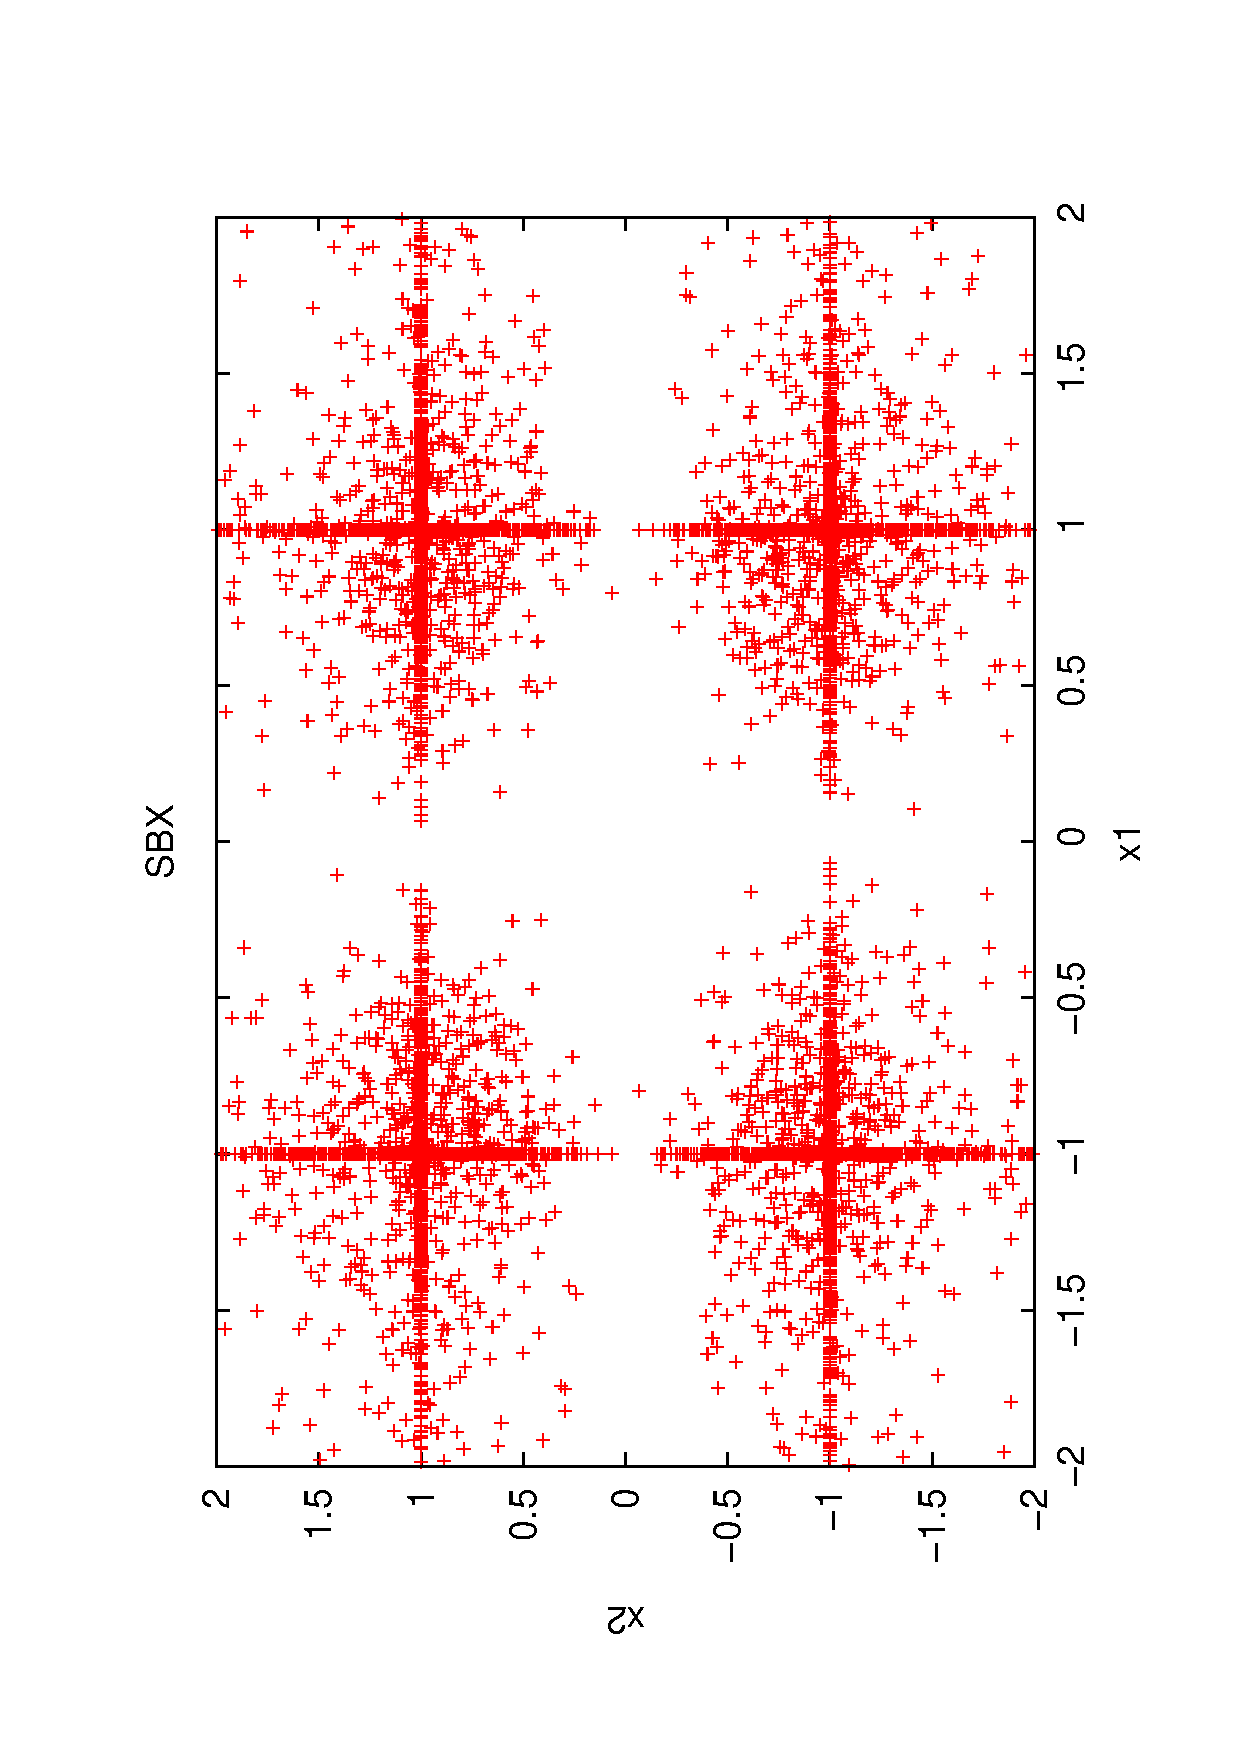
\includegraphics[width=0.24\textwidth]{img/Operadores/SBX_eta_2.png}  %&
   \includegraphics[width=0.24\textwidth]{img/Operadores/SBX_eta_20.png} 
\end{tabular}
\caption{Simulation of the \SBX{} operator sampling $10,000$ children values, the parents are located in $P_1=(-1.0, -1.0)$ and $P_2=(1.0, 1.0)$. The left and right are with a distribution index of $2$ and $20$ respectively.}
\label{fig:Simulation_Case_3}
\end{figure}

The second key issue is that after generating the two child values with the \SBX{} distribution, such values
are interchanged with a fixed probability that is usually set to $0.5$, i.e. the value closer to parent $p_1$ is
not always inherited by $c_1$.
%
This is a feature that is not usually discussed but it is important for the obtained performance.
%
In some contexts this probability is known as ``Variable uniform crossover probability'' 
\cite{tuvsar2007differential} or ``Discrete Recombination'' \cite{muhlenbein1993predictive}.
%
Since in multi-objective optimization more diversity is maintained these swaps might produce a high disruptive operator.
%
In fact, in some sense due to this action it is not so clear that \SBX{} can be categorized as a parent-centric operator.
%
These interchanges between the children has the effect of performing multiple ``reflections'' in the search space.
%
When increasing the dimensions of the decision variables the number of regions covered increases exponentially 
as is illustrated in Figure \ref{fig:Simulations_Index_20} where cases with two and three decision variables are taken into account.
%
Note also that this feature has a considerable effect on the distance between parents and offspring.

Finally, the last component is the distribution index, which is probably the most well known feature of the \SBX{}.
%
A low index results in greater exploration levels.
%
In fact, a distribution index equal to one has a similar effect to the Fuzzy Recombination Operator \cite{voigt1995fuzzy}.
%
The effect of applying different indexes is illustrated in Figure~\ref{fig:Simulation_Case_3} where the left side
considers a low index value whereas the right side takes into account a higher index value, which creates 
new candidate solutions that are more similar to the parents.
%

The \SBX{} implementation is shown in Algorithm \ref{alg:SBX_Operator}.
%
This pseudocode is based on the implementation that is integrated in the NSGA-II code published by Deb et al. \cite{Joel:NSGAII} and which
is the most popular variant nowadays.
%
As an input it requires two parents ($P_1$ and $P_2$) and it creates two children ($C_1$ and $C_2$).
%
The first and second key components commented previously correspond to the lines 5 and 8, respectively. 
%
As is usual, for the basic case, \SBX{} is configured with $\delta_1 = \delta_2 = 0.5$ and $\eta_c = 20$.
%
It is important take into account that this implementation does not consider the dimension of the decision variables 
or the stopping criteria to set any of its internal parameters.

\subsection{Propuesta}

Based on the previous analyses and with the aim of inducing an appropriate balance between 
exploration and intensification, the following modifications are proposed.
%
First, the probability to modify a variable ($\delta_1$) is dynamically
modified during the execution.
%
The rationality behind this modification is to increase the exploration capability in the initial stages
by altering simultaneously several variables and then, as the evolution proceeds reduce the number of variables
that are modified.
%
The value of $\delta_1$ is changed in base of a linear decreasing model, where initially it is fixed to $1.0$ and 
then it is decreased so that at the half of total generations is equal to $0.5$.
%
This last value is maintained until the end of the execution, i.e. from the half of the execution it behaves as the 
traditional \SBX{} implementation.
%
Equation (\ref{eqn:linear}) is the one used to set the value of $\delta_1$, where $G_{Elapsed}$ is the current generation 
and $G_{End}$ is the total number of generations.

In a similar way, the second change is related to the probability of performing reflections ($1 - \delta_2$).
%
In this case $\delta_2$ is also updated as in Equation (\ref{eqn:linear}), meaning that the probability of performing
a reflection increases from $0.0$ to $0.5$ during the execution.
%
This modification is performed with the aim of avoiding the disruptive behavior of interchanging the variables at the
first generations because this might result in very drastic modifications.
%
Once that the individuals converge to certain degree it might make more sense to perform such reflections.
%
Thus, this probability is increased to $0.5$ which is the value used in the standard implementation of \SBX{}.

\begin{equation}\label{eqn:linear}
	\delta_1 = \delta_2 = max \left (0.5, 1.0 - \frac{G_{Elapsed}}{G_{End}} \right )
\end{equation}

Finally, the distribution index is also changed during the execution. 
%
At the first stages a low distribution index is induced with the aim of increasing the exploration capabilities 
of \SBX{}.
%
Then, it is linearly incremented which has the effect of closing the distribution curve, meaning that more intensification is
promoted.
%
The linear increment is governed by Equation (\ref{eqn:index_eta}), meaning that the distribution index is altered
from $2$ to $22$.
%
Note that modifications similar to this last one have been explored previously 
\cite{zitzler1999multiobjective}, \cite{hamdan2012distribution}.
%

\begin{equation}\label{eqn:index_eta}
 \eta_c = 2 + 20 \times \left ( \frac{G_{Elapsed}}{G_{End}} \right)
\end{equation}

\subsection{Resultados}

\begin{table}[t]
\centering
\scriptsize
\caption{References points for the HV indicator}
\label{tab:ReferencePoints}
\begin{tabular}{cc}
\hline
\textbf{Instances} & \textbf{Reference Point} \\ \hline
WFG1-WFG9 & $[2.1, ...,2m+0.1]$ \\
DTLZ 1, 2, 4 & $[1.1, ..., 1.1]$ \\
DTLZ 3, 5, 6 & $[3, ..., 3]$ \\
DTLZ7 & $[1.1, ..., 1.1, 2m]$ \\
UF 1-10 & $[2, ..., 2]$ \\ \hline
\end{tabular}
\end{table}


% Please add the following required packages to your document preamble:
% \usepackage{multirow}
% \usepackage{graphicx}
\begin{table*}[t]
\centering

\caption{Statistical Information of Metrics with two objectives}
\label{tab:Metrics_2}
\resizebox{\textwidth}{!}{%
\begin{tabular}{|c|c|c|c|c|c|c|c|c|c|c|c|c|c|c|c|c|c|c|}
\hline
\multirow{2}{*}{} & \multicolumn{6}{c|}{NSGA-II} & \multicolumn{6}{c|}{MOEA/D} & \multicolumn{6}{c|}{SMS-EMOA} \\ \cline{2-19} 
 & 1 & 2 & 3 & 4 & 5 & DE & 1 & 2 & 3 & 4 & 5 & DE & 1 & 2 & 3 & 4 & 5 & DE \\ \hline
Average HV & 0.88 & 0.90 & 0.90 & 0.91 & 0.93 & \textbf{0.94} & 0.87 & 0.87 & 0.87 & 0.90 & \textbf{0.91} & \textbf{0.91} & 0.88 & 0.89 & 0.87 & 0.91 & 0.92 & \textbf{0.93} \\ \hline
%Best Counts HV & 2 & 1 & 0 & 1 & 8 & \textbf{11} & 2 & 0 & 2 & 2 & 8 & \textbf{9} & 0 & 1 & 1 & 5 & 6 & \textbf{10} \\ \hline
%\multicolumn{1}{|l|}{Average Best Difference HV} & \multicolumn{1}{l|}{0.068} & \multicolumn{1}{l|}{0.057} & \multicolumn{1}{l|}{0.053} & \multicolumn{1}{l|}{0.039} & \multicolumn{1}{l|}{0.019} & \multicolumn{1}{l|}{\textbf{0.017}} & \multicolumn{1}{l|}{0.053} & \multicolumn{1}{l|}{0.048} & \multicolumn{1}{l|}{0.049} & \multicolumn{1}{l|}{0.024} & \multicolumn{1}{l|}{\textbf{0.013}} & \multicolumn{1}{l|}{0.014} & \multicolumn{1}{l|}{0.074} & \multicolumn{1}{l|}{0.064} & \multicolumn{1}{l|}{0.081} & \multicolumn{1}{l|}{0.045} & \multicolumn{1}{l|}{0.028} & \multicolumn{1}{l|}{\textbf{0.019}} \\ \hline
Average IGD+ & 0.12 & 0.09 & 0.11 & 0.07 & 0.06 & \textbf{0.05} & 0.14 & 0.12 & 0.14 & 0.09 & 0.08 & \textbf{0.07} & 0.13 & 0.11 & 0.14 & 0.08 & 0.07 & \textbf{0.05} \\ \hline
%Best Counts IGD+ & 2 & 1 & 1 & 1 & 8 & \textbf{10} & 3 & 0 & 2 & 3 & 6 & \textbf{9} & 0 & 2 & 0 & 3 & \textbf{9} & \textbf{9} \\ \hline
%\multicolumn{1}{|l|}{Average Best Difference IGD+} & \multicolumn{1}{l|}{0.086} & \multicolumn{1}{l|}{0.052} & \multicolumn{1}{l|}{0.077} & \multicolumn{1}{l|}{0.035} & \multicolumn{1}{l|}{0.021} & \multicolumn{1}{l|}{\textbf{0.016}} & \multicolumn{1}{l|}{0.075} & \multicolumn{1}{l|}{0.059} & \multicolumn{1}{l|}{0.072} & \multicolumn{1}{l|}{0.025} & \multicolumn{1}{l|}{0.019} & \multicolumn{1}{l|}{\textbf{0.008}} & \multicolumn{1}{l|}{0.093} & \multicolumn{1}{l|}{0.071} & \multicolumn{1}{l|}{0.101} & \multicolumn{1}{l|}{0.038} & \multicolumn{1}{l|}{0.030} & \multicolumn{1}{l|}{\textbf{0.017}} \\ \hline
\end{tabular}%
}
\end{table*}

% Please add the following required packages to your document preamble:
% \usepackage{multirow}
% \usepackage{graphicx}
\begin{table*}[t]
\centering
\caption{Statistical Information of Metrics with three objectives}
\label{tab:Metrics_3}
\resizebox{\textwidth}{!}{%
\begin{tabular}{|c|c|c|c|c|c|c|c|c|c|c|c|c|c|c|c|c|c|c|}
\hline
\multirow{2}{*}{} & \multicolumn{6}{c|}{NSGA-II} & \multicolumn{6}{c|}{MOEA/D} & \multicolumn{6}{c|}{SMS-EMOA} \\ \cline{2-19} 
 & 1 & 2 & 3 & 4 & 5 & DE & 1 & 2 & 3 & 4 & 5 & DE & 1 & 2 & 3 & 4 & 5 & DE \\ \hline
Average HV & \textbf{0.87} & 0.84 & \textbf{0.87} & \textbf{0.87} & \textbf{0.87} & 0.85 & 0.84 & 0.84 & 0.84 & \textbf{0.86} & \textbf{0.86} & 0.85 & 0.90 & 0.89 & 0.88 & \textbf{0.91} & \textbf{0.91} & \textbf{0.91} \\ \hline
%Best Counts HV & 1 & 2 & 1 & 4 & 4 & \textbf{7} & 1 & 2 & 1 & 2 & 5 & \textbf{8} & 3 & 2 & 0 & 2 & 5 & \textbf{7} \\ \hline
%\multicolumn{1}{|l|}{Average Best Difference HV} & \multicolumn{1}{l|}{0.019} & \multicolumn{1}{l|}{0.047} & \multicolumn{1}{l|}{0.020} & \multicolumn{1}{l|}{\textbf{0.014}} & \multicolumn{1}{l|}{\textbf{0.014}} & \multicolumn{1}{l|}{0.032} & \multicolumn{1}{l|}{0.036} & \multicolumn{1}{l|}{0.041} & \multicolumn{1}{l|}{0.038} & \multicolumn{1}{l|}{0.016} & \multicolumn{1}{l|}{\textbf{0.013}} & \multicolumn{1}{l|}{0.027} & \multicolumn{1}{l|}{0.038} & \multicolumn{1}{l|}{0.038} & \multicolumn{1}{l|}{0.049} & \multicolumn{1}{l|}{\textbf{0.019}} & \multicolumn{1}{l|}{0.027} & \multicolumn{1}{l|}{\textbf{0.019}} \\ \hline
Average IGD+ & 0.13 & 0.16 & 0.13 & \textbf{0.12} & \textbf{0.12} & 0.13 & 0.15 & 0.14 & 0.15 & \textbf{0.11} & \textbf{0.11} & 0.13 & 0.11 & 0.11 & 0.13 & \textbf{0.09} & \textbf{0.09} & 0.13 \\ \hline
%Best Counts IGD+ & 0 & 2 & 2 & 4 & 3 & \textbf{8} & 2 & 2 & 0 & 2 & 4 & \textbf{9} & 1 & 3 & 0 & 3 & 5 & \textbf{7} \\ \hline
%\multicolumn{1}{|l|}{Average Best Difference IGD+} & \multicolumn{1}{l|}{0.029} & \multicolumn{1}{l|}{0.061} & \multicolumn{1}{l|}{0.027} & \multicolumn{1}{l|}{0.023} & \multicolumn{1}{l|}{\textbf{0.020}} & \multicolumn{1}{l|}{0.032} & \multicolumn{1}{l|}{0.053} & \multicolumn{1}{l|}{0.048} & \multicolumn{1}{l|}{0.053} & \multicolumn{1}{l|}{\textbf{0.015}} & \multicolumn{1}{l|}{\textbf{0.015}} & \multicolumn{1}{l|}{0.030} & \multicolumn{1}{l|}{0.047} & \multicolumn{1}{l|}{0.040} & \multicolumn{1}{l|}{0.062} & \multicolumn{1}{l|}{\textbf{0.020}} & \multicolumn{1}{l|}{0.024} & \multicolumn{1}{l|}{0.069} \\ \hline
\end{tabular}%
}
\end{table*}
\begin{table*}[t]
\centering
\caption{Summary of Statistical Tests}
\label{tab:statistical_Tests}
\begin{tabular}{|c|c|c|c|c|c|c|c|c|c|c|c|c|c|c|c|}
\hline
\multicolumn{16}{|c|}{NSGA-II} \\ \hline
 & \multicolumn{3}{c|}{1} & \multicolumn{3}{c|}{2} & \multicolumn{3}{c|}{3} & \multicolumn{3}{c|}{4} & \multicolumn{3}{c|}{5} \\ \hline
 & $\uparrow$ & $\downarrow$ & $\longleftrightarrow$ & $\uparrow$ & $\downarrow$ & $\longleftrightarrow$ & $\uparrow$ & $\downarrow$ & $\longleftrightarrow$ & $\uparrow$ & $\downarrow$ & $\longleftrightarrow$ & $\uparrow$ & $\downarrow$ & $\longleftrightarrow$ \\ \hline
\textbf{HV-2obj} & 16 & 29 & 47 & 6 & 61 & 25 & 28 & 19 & 45 & 31 & 23 & 38 & \textbf{54} & 3 & 35 \\ \hline
\textbf{HV-3obj} & 15 & 19 & 42 & 12 & 50 & 14 & 17 & 15 & 44 & \textbf{33} & 10 & 33 & 26 & 9 & 41 \\ \hline
\textbf{IGD-2obj} & 14 & 30 & 48 & 4 & 60 & 28 & 25 & 17 & 50 & 33 & 19 & 40 & \textbf{52} & 2 & 38 \\ \hline
\textbf{IGD-3obj} & 14 & 18 & 44 & 13 & 44 & 19 & 18 & 15 & 43 & \textbf{33} & 15 & 28 & 23 & 9 & 44 \\ \hline
% \end{tabular}
% \end{table*}

% \begin{table*}[]
% \centering
% \caption{My caption}
% \label{my-label}
% \begin{tabular}{|c|c|c|c|c|c|c|c|c|c|c|c|c|c|c|c|}
\hline
\hline
\multicolumn{16}{|c|}{MOEA/D} \\ \hline
 & \multicolumn{3}{c|}{1} & \multicolumn{3}{c|}{2} & \multicolumn{3}{c|}{3} & \multicolumn{3}{c|}{4} & \multicolumn{3}{c|}{5} \\ \hline
 & $\uparrow$ & $\downarrow$ & $\longleftrightarrow$ & $\uparrow$ & $\downarrow$ & $\longleftrightarrow$ & $\uparrow$ & $\downarrow$ & $\longleftrightarrow$ & $\uparrow$ & $\downarrow$ & $\longleftrightarrow$ & $\uparrow$ & $\downarrow$ & $\longleftrightarrow$ \\ \hline
\textbf{HV-2obj} & 15 & 33 & 44 & 10 & 60 & 22 & 25 & 26 & 41 & 39 & 18 & 35 & \textbf{57} & 9 & 26 \\ \hline
\textbf{HV-3obj} & 10 & 22 & 44 & 12 & 39 & 25 & 11 & 19 & 46 & 24 & 10 & 42 & \textbf{38} & 5 & 33 \\ \hline
\textbf{IGD-2obj} & 16 & 31 & 45 & 9 & 60 & 23 & 23 & 27 & 42 & 37 & 17 & 38 & \textbf{57} & 7 & 28 \\ \hline
\textbf{IGD-3obj} & 12 & 22 & 42 & 13 & 43 & 20 & 13 & 24 & 39 & 30 & 9 & 37 & \textbf{40} & 10 & 26 \\ \hline
% \end{tabular}
% \end{table*}

% \begin{table*}[]
% \centering
% \caption{My caption}
% \label{my-label}
% \begin{tabular}{|c|c|c|c|c|c|c|c|c|c|c|c|c|c|c|c|}
\hline
\hline
\multicolumn{16}{|c|}{SMS-EMOA} \\ \hline
 & \multicolumn{3}{c|}{1} & \multicolumn{3}{c|}{2} & \multicolumn{3}{c|}{3} & \multicolumn{3}{c|}{4} & \multicolumn{3}{c|}{5} \\ \hline
 & $\uparrow$ & $\downarrow$ & $\longleftrightarrow$ & $\uparrow$ & $\downarrow$ & $\longleftrightarrow$ & $\uparrow$ & $\downarrow$ & $\longleftrightarrow$ & $\uparrow$ & $\downarrow$ & $\longleftrightarrow$ & $\uparrow$ & $\downarrow$ & $\longleftrightarrow$ \\ \hline
\textbf{HV-2obj} & 9 & 35 & 48 & 7 & 43 & 42 & 16 & 31 & 45 & 41 & 9 & 42 & \textbf{53} & 8 & 31 \\ \hline
\textbf{HV-3obj} & 7 & 21 & 48 & 9 & 35 & 32 & 13 & 21 & 42 & 27 & 6 & 43 & \textbf{31} & 4 & 41 \\ \hline
\textbf{IGD-2obj} & 10 & 34 & 48 & 15 & 48 & 29 & 12 & 33 & 47 & 41 & 12 & 39 & \textbf{55} & 6 & 31 \\ \hline
\textbf{IGD-3obj} & 8 & 20 & 48 & 13 & 30 & 33 & 9 & 19 & 48 & 22 & 5 & 49 & \textbf{27} & 5 & 44 \\ \hline
\end{tabular}
\end{table*}


This section is devoted to analyze the results obtained with the dynamic variants of \SBX{} (\DSBX{}).
%
The novel crossover operator was integrated with \NSGAII{}, \MOEAD{} and \SMSEMOA{}.
%
First, three variants that alter only one of each of the components previously discussed are analyzed.
%
Then, a case that alters two of them simultaneously is taken into account.
%
The WFG \cite{Joel:WFG}, DTLZ \cite{Joel:DTLZ_2} and UF \cite{zhang2009performance} test problems have been used for our purpose.
%
Our experimental validation also includes the variant of Differential Evolution known as DEMO~\cite{tuvsar2007differential}
with the aim of comparing our extension of \SBX{} with other well-known operators.

Given that all the methods are stochastic algorithms, each execution was repeated $35$ times with different seeds.
%
The common configuration in all of them was the following: the stopping criterion was set to $25,000$ generations, 
the population size was fixed to 100, WFG test problems were configured with two and three objectives, and 24 variables
were considered, where 20 of them are distance parameters and 4 of them are position parameters.
%
In the case of the DTLZ test instances, the number of decision variables were set to $n=M+r-1$, where $r=\{5, 10, 20\}$ 
for DTLZ1, DTLZ2 to DTLZ6 and DTLZ7 respectively, as is suggested in\cite{Joel:DTLZ_2}.  
% 
In the UF benchmark set the number of decision variables were set to 10.
%
Finally, the polynomial mutation was used with a mutation probability equal to $1/n$ and with a distribution index equal to 50, 
whereas for the cases that used the \SBX{}, the crossover probability was set to $0.9$ and the distribution index
was set to 20.
%
The additional parameterization of each algorithm was as follows:
\begin{itemize}
\item \textbf{DEMO}: CR = 0.3 and F = 0.5.
\item \textbf{SMS-EMOA}: offset = 100.
\item \textbf{MOEA/D}: size of neighborhood = 10, max updates by sub-problem (nr) = 2 and $\delta = 0.9$.
\end{itemize}

In order to compare the fronts obtained by the different methods the 
normalized hypervolume (HV) and IGD+ was taken into account.
%
The reference points used for the hypervolume indicator are shown in the Table \ref{tab:ReferencePoints} 
and are similar to the ones used in \cite{Joel:Kuhn_Munkres, Joel:OperatorAHX}.

In order to statistically compare the results (IGD+ and HV values), the following statistical tests were performed. 
%
First a Shapiro-Wilk test was performed to check whatever or not the values of the results followed a Gaussian distribution. 
%
If, so, the Levene test was used to check for the homogeneity of the variances. 
%
If samples had equal variance, an ANOVA test was done; if not, a Welch test was performed. 
%
For non-Gaussian distributions, the nonparametric Kruskal-Wallis test was used to test whether samples are drawn 
from the same distribution. 
%
An algorithm $X$ is said to win algorithm $Y$ when the differences between them are statistically significant, and
the mean and median obtained by $X$ are higher (in HV) or lower (in IGD+) than the mean and median achieved by $Y$.


\subsection{Analysis of isolated components}

In this section we discuss about the independent effect of each component that is dynamically modified.
%
%Particularly, the jMetalcpp framework \cite{Joel:jMetal}  was used to perform our executions.
%
%Taking into account the stochastic behavior of MOEAs, $35$ independent executions were run.
%
%In all of them, the stopping criteria was set to $25,000$ generations and the size of the population was fixed to $100$.
%
The effect of each component is analyzed through four cases, based in the Algorithm \ref{alg:SBX_Operator}.
%
Each case is described as follows:

\begin{itemize}
\item \textbf{Case 1}: The standard SBX operator where $\delta_1 = \delta_2 = 0.5$ and $\eta_c = 20$.
\item \textbf{Case 2}: The value $\delta_1$ is updated according to Equation~(\ref{eqn:linear}),  $\delta_2=0.5$ and $\eta_c = 20$.
\item \textbf{Case 3}: The value $\delta_2$ is updated according to Equation~(\ref{eqn:linear}), $\delta_1=0.5$ and $\eta_c = 20$.
\item \textbf{Case 4}: The distribution index is updated according to Equation~(\ref{eqn:index_eta}), $\delta_1=\delta_2=0.5$.
\end{itemize}


In order to analyze the performance of each Case (Case 5 is discussed later), Tables \ref{tab:Metrics_2} and
\ref{tab:Metrics_3} shows information about the Normalized Hyper-volume 
(HV)~\cite{zitzler1999multiobjective} and about the Inverted Generational Distance Plus (IGD+)~\cite{Joel:IGDPlus_And_GDPlus}.
%
Specifically, the mean of the HV and IGD+ for all considered problems are shown for two and three objectives.
%
It is clear that case 4 outperforms case 1, case 2 and case 3 both with two and three objectives in all the tested algorithms.
%
Therefore, increasing the distribution index during the execution seems to be the most beneficial action.
%
This occurs because the initially open distribution curve leads to a higher degree of exploration, whereas as the evolution
proceeds more intensification is promoted.
%
On the other hand, case 2 presented a lower performance than case 1 when taking into account three objectives.
%
Thus, it seems that altering almost all the variables convert the new approach into a too disruptive operator.
%
Perhaps, altering $\delta_1$ in a different way might provide better results, but this is left as a future work.

Previous analyses are only based on the mean obtained for all the problems.
%
However, depending on the problem the performance might vary.
%
This is analyzed in the following section.
%
Additionally, more detailed results are available\footnote{https:\//\//github.com\//joelchaconcastillo\//SBX\_CEC2018.}.


\subsection{Simultaneous modification of several components}

Based on the previously discussed results, a variant of the \SBX{} is proposed where the case 3 and case 4 are mixed, 
i.e. both $\delta_2$ and the distribution index are updated dynamically.
%
Since case 2 did not report significant benefits, the updating mechanism for $\delta_1$ was discarded.
%
Specifically in our case 5, Algorithm \ref{alg:SBX_Operator} is configured as follows.
%
The parameter $\delta_1$ is fixed to $0.5$, i.e. in a similar way than the standard \SBX{}.
%
Following the case 3, $\delta_2$ is updated according to Equation~(\ref{eqn:linear}).
%
Finally, according to case 4 $\eta_c$ is updated in base of Equation~(\ref{eqn:index_eta}).

Attending to the mean HV and IGD+ obtained by the case 5 (see Tables~\ref{tab:Metrics_2} and \ref{tab:Metrics_3})
it is clear that integrating case 3 and case 4 is beneficial.
%
The advantages are clearer in the case of two objectives, whereas in the case of three objectives, case 4
and case 5 are similar in terms of mean performance.
%
Moreover, results attained with case 5 are superior to the ones obtained with \DE{} in three objectives, whereas
when using the traditional \SBX{} results deteriorate.
%
Thus, when properly configuring a \DSBX{} results similar or superior to DEMO could be obtained.

Finally, since previous analyses only consider the mean among all the benchmark problems, an additional analyses
was developed to better understand the contributions of the different cases.
%
Particularly, pair-wise statistical tests among all the five cases that consider \SBX{} and \DSBX{} were carried out.
%
This was performed independently for \NSGAII{}, \MOEAD{} and \SMSEMOA{}.
%
Results of these statistical tests are shown in Table~\ref{tab:statistical_Tests}.
%
For each algorithm and case, the column ``$\uparrow$'' reports the number of comparisons where the statistical tests 
confirmed the superiority of the corresponding case, whereas the column ``$\downarrow$'' reports the number of cases 
where it was inferior and ``$\longleftrightarrow$'' indicates the number of comparisons where 
differences were not statistically significant.
%%
The advantages of case 5 are quite clear.
%
Only in the case of \NSGAII{} with three objectives, case 4 could outperform the results obtained by case 5.
%
Thus, by properly combining several dynamic modification, results can be improved further.
%
Moreover, results confirm the advantages of our proposals when compared to the standard \SBX{} (case 1).
%
The only case that is not clearly superior to the standard \SBX{} is the case number 2, as it was previously discussed.
%

%This might occurs for the ranking mechanism of this MOEA.
%
%Since that the NSGA-II applies a binary tournament selection based in dominance concept and crowding procedure, thus an appropriate level of diversity is maintained.
%
%As result some promising regions are reached.

%
%Although that with three objective the Case 4 and our proposal have similar average results.
%
%The average difference with the best indicates that our proposal is mostly closest to the best values.
%
%This since that it shows $0.020$ in the ``Average Best Difference'' IGD+ against the Case 4 with $0.023$.
%
%Also, inspecting the statistical tests, the Case 4 has more loses than our proposal ($10$ against $9$ and $15$ against $9$) of the HV and IGD+ respectively.
%
%However, the MOEA/D and SMS-EMOA which are more elitist algorithms and do not consider the dominance concept at all, are not affected in this sense.
%
%Anyway, our proposal and the Case 3 reports significantly better results that the normal SBX (Case 1), in fact this could evidence that variate the distribution index among the execution has an important effect.




%In the Table \ref{tab:statistical_Tests} is showed a summary of the statistical tests, where are considered the HV and IGD+ both in two and three objectives.
%
%Based in the statistical tests (Table \ref{tab:statistical_Tests}), the Case 4 which correspond to the dynamic distribution index, yield better results than Case 1, Case 2 and Case 3.
%
%
%In the second place is the Case 3, it increases the probability of interchange a variable based in a linear model, this might occurs since that at the first stages are avoided disruptive modifications.
%
%Therefore, the promising regions are not adequately explored, although that this case does not yield the best results, it still outperforms the standard SBX (Case 1).
%
%Also can be noticed that the results of the HV are similar that with the IGD+.
%





%Although that the DE variants provides better average results than our proposal considering two objective, our proposal provides near solutions to the best, showing its stability.
%
%Also according the number of objectives increase to three our proposal provides the best results.
%
%The main reason is that DE is seriously deteriorated as the number of objectives increases, also it converges in a fast way, since it incorporates an aggressive selection operator.
%

%Despite the fact that DE variants have high ``Best Count'' values, in average it is improved by the Case 4 and Case 5, this might occurs because DE is directly influenced by the probability crossover ($CR$) and the mutation factor ($F$), therefore in some instances the DE variants attained the best results, and in other instances the solutions are far from the Pareto front.
%

%On the other hand, our proposal shows a robust behavior in the state-of-the-art MOEAs, in fact the ``Average Best Difference'' is low both with two objectives and three objectives that confirms the stability and superiority of our proposal.
%
% % Please add the following required packages to your document preamble:
% % \usepackage{multirow}
% % \usepackage{graphicx}
% \begin{table*}[]
% \centering
% \caption{Statistical Information of Metrics}
% \label{my-label}
% \resizebox{\textwidth}{!}{%
% \begin{tabular}{|l|c|c|c|c|c|c|c|c|c|c|c|c|c|c|c|c|c|c|c|}
% \hline
% \multicolumn{2}{|l|}{\multirow{2}{*}{}} & \multicolumn{6}{c|}{NSGA-II} & \multicolumn{6}{c|}{MOEA/D} & \multicolumn{6}{c|}{SMS-EMOA} \\ \cline{3-20} 
% \multicolumn{2}{|l|}{} & 1 & 2 & 3 & 4 & 5 & 6 & 1 & 2 & 3 & 4 & 5 & 6 & 1 & 2 & 3 & 4 & 5 & 6 \\ \hline
% \multirow{6}{*}{2 Objectives} & Average HV & 0.88 & 0.90 & 0.90 & 0.91 & 0.93 & \textbf{0.94} & 0.87 & 0.87 & 0.87 & 0.90 & \textbf{0.91} & \textbf{0.91} & 0.88 & 0.89 & 0.87 & 0.91 & 0.92 & \textbf{0.93} \\ \cline{2-20} 
%  & Best Counts HV & 2 & 1 & 0 & 1 & 8 & \textbf{11} & 2 & 0 & 2 & 2 & 8 & \textbf{9} & 0 & 1 & 1 & 5 & 6 & \textbf{10} \\ \cline{2-20} 
%  & \multicolumn{1}{l|}{Average Best Difference HV} & \multicolumn{1}{l|}{0.068} & \multicolumn{1}{l|}{0.057} & \multicolumn{1}{l|}{0.053} & \multicolumn{1}{l|}{0.039} & \multicolumn{1}{l|}{0.019} & \multicolumn{1}{l|}{\textbf{0.017}} & \multicolumn{1}{l|}{0.053} & \multicolumn{1}{l|}{0.048} & \multicolumn{1}{l|}{0.049} & \multicolumn{1}{l|}{0.024} & \multicolumn{1}{l|}{\textbf{0.013}} & \multicolumn{1}{l|}{0.014} & \multicolumn{1}{l|}{0.074} & \multicolumn{1}{l|}{0.064} & \multicolumn{1}{l|}{0.081} & \multicolumn{1}{l|}{0.045} & \multicolumn{1}{l|}{0.028} & \multicolumn{1}{l|}{\textbf{0.019}} \\ \cline{2-20} 
%  & Average IGD+ & 0.12 & 0.09 & 0.11 & 0.07 & 0.06 & \textbf{0.05} & 0.14 & 0.12 & 0.14 & 0.09 & 0.08 & \textbf{0.07} & 0.13 & 0.11 & 0.14 & 0.08 & 0.07 & \textbf{0.05} \\ \cline{2-20} 
%  & Best Counts IGD+ & 2 & 1 & 1 & 1 & 8 & \textbf{10} & 3 & 0 & 2 & 3 & 6 & \textbf{9} & 0 & 2 & 0 & 3 & \textbf{9} & \textbf{9} \\ \cline{2-20} 
%  & \multicolumn{1}{l|}{Average Best Difference IGD+} & \multicolumn{1}{l|}{0.086} & \multicolumn{1}{l|}{0.052} & \multicolumn{1}{l|}{0.077} & \multicolumn{1}{l|}{0.035} & \multicolumn{1}{l|}{0.021} & \multicolumn{1}{l|}{\textbf{0.016}} & \multicolumn{1}{l|}{0.075} & \multicolumn{1}{l|}{0.059} & \multicolumn{1}{l|}{0.072} & \multicolumn{1}{l|}{0.025} & \multicolumn{1}{l|}{0.019} & \multicolumn{1}{l|}{\textbf{0.008}} & \multicolumn{1}{l|}{0.093} & \multicolumn{1}{l|}{0.071} & \multicolumn{1}{l|}{0.101} & \multicolumn{1}{l|}{0.038} & \multicolumn{1}{l|}{0.030} & \multicolumn{1}{l|}{\textbf{0.017}} \\ \hline
% \multirow{6}{*}{3 Objectives} & Average HV & \textbf{0.87} & 0.84 & \textbf{0.87} & \textbf{0.87} & \textbf{0.87} & 0.85 & 0.84 & 0.84 & 0.84 & \textbf{0.86} & \textbf{0.86} & 0.85 & 0.90 & 0.89 & 0.88 & \textbf{0.91} & \textbf{0.91} & \textbf{0.91} \\ \cline{2-20} 
%  & Best Counts HV & 1 & 2 & 1 & 4 & 4 & \textbf{7} & 1 & 2 & 1 & 2 & 5 & \textbf{8} & 3 & 2 & 0 & 2 & 5 & \textbf{7} \\ \cline{2-20} 
%  & \multicolumn{1}{l|}{Average Best Difference HV} & \multicolumn{1}{l|}{0.019} & \multicolumn{1}{l|}{0.047} & \multicolumn{1}{l|}{0.020} & \multicolumn{1}{l|}{\textbf{0.014}} & \multicolumn{1}{l|}{\textbf{0.014}} & \multicolumn{1}{l|}{0.032} & \multicolumn{1}{l|}{0.036} & \multicolumn{1}{l|}{0.041} & \multicolumn{1}{l|}{0.038} & \multicolumn{1}{l|}{0.016} & \multicolumn{1}{l|}{\textbf{0.013}} & \multicolumn{1}{l|}{0.027} & \multicolumn{1}{l|}{0.038} & \multicolumn{1}{l|}{0.038} & \multicolumn{1}{l|}{0.049} & \multicolumn{1}{l|}{\textbf{0.019}} & \multicolumn{1}{l|}{0.027} & \multicolumn{1}{l|}{\textbf{0.019}} \\ \cline{2-20} 
%  & Average IGD+ & 0.13 & 0.16 & 0.13 & \textbf{0.12} & \textbf{0.12} & 0.13 & 0.15 & 0.14 & 0.15 & \textbf{0.11} & \textbf{0.11} & 0.13 & 0.11 & 0.11 & 0.13 & \textbf{0.09} & \textbf{0.09} & 0.13 \\ \cline{2-20} 
%  & Best Counts IGD+ & 0 & 2 & 2 & 4 & 3 & \textbf{8} & 2 & 2 & 0 & 2 & 4 & \textbf{9} & 1 & 3 & 0 & 3 & 5 & \textbf{7} \\ \cline{2-20} 
%  & \multicolumn{1}{l|}{Average Best Difference IGD+} & \multicolumn{1}{l|}{0.029} & \multicolumn{1}{l|}{0.061} & \multicolumn{1}{l|}{0.027} & \multicolumn{1}{l|}{0.023} & \multicolumn{1}{l|}{\textbf{0.020}} & \multicolumn{1}{l|}{0.032} & \multicolumn{1}{l|}{0.053} & \multicolumn{1}{l|}{0.048} & \multicolumn{1}{l|}{0.053} & \multicolumn{1}{l|}{\textbf{0.015}} & \multicolumn{1}{l|}{\textbf{0.015}} & \multicolumn{1}{l|}{0.030} & \multicolumn{1}{l|}{0.047} & \multicolumn{1}{l|}{0.040} & \multicolumn{1}{l|}{0.062} & \multicolumn{1}{l|}{\textbf{0.020}} & \multicolumn{1}{l|}{0.024} & \multicolumn{1}{l|}{0.069} \\ \hline
% \end{tabular}%
% }
% \end{table*}


% \begin{figure}[!t]
% \centering
% \includegraphics[scale=0.25,angle=-90]{img/bar_HV_2obj.eps}
% \caption{Average of normalized hypervolume considering all the instances and two objective.}
% \label{fig_sim}
% \end{figure}
% \begin{figure}[]
% \centering
% \includegraphics[scale=0.25,angle=-90]{img/bar_IGD_2obj.eps}
% \caption{Average of Inverted Generalized Distance Plus (IGD+) considering all the instances and two objective.}
% \label{fig_sim}
% \end{figure}

% \begin{figure}[!t]
% \centering
% \includegraphics[scale=0.25,angle=-90]{img/bar_HV_3obj.eps}
% \caption{Average of normalized hypervolume considering all the instances and three objective.}
% \label{fig_sim}
% \end{figure}
% \begin{figure}[]
% \centering
% \includegraphics[scale=0.25,angle=-90]{img/bar_IGD_3obj.eps}
% \caption{Average of Inverted Generalized Distance Plus (IGD+) considering all the instances and three objective.}
% \label{fig_sim}
% \end{figure}




\section{Conclusiones y trabajo futuro}
\label{sec:Conclusion}
La convergencia prematura es una de las debilidades más importantes de los \EAS{}.
%
Una de las formas de lidiar con este problema consiste en inducir un balanceo adecuado entre exploración e intensificación.
%
Sin embargo, obtener este balanceo no es una tarea trivial debido a que cada problema de optimización tiene características distintas y por
ello han surgido numerosos esquemas para tratar esta problemática.
%
Con base en esto se han desarrollado varias taxonomías con el propósito de clasificar las diferentes formas en que se puede preservar y promover la diversidad.
%
En este trabajo, con el fin de ilustrar como se pueden realizar diseños de \EAS{} que tomen en cuenta el balanceo entre exploración e intensificación
se presentan dos ejemplos.
%
De forma general, las propuestas establecen un comportamiento dinámico de algún componente del \EA{} teniendo en cuenta para ello el criterio de paro 
y el instante en que se encuentra la ejecución.
%
Así, se obtuvo un balanceo adecuado en el que en las primeras fases se promueve más exploración y en las últimas se promueve más la intensificación. 
%
De modo más específico, en la primera propuesta se modifica evolución diferencial por medio de una nueva fase de reemplazo con el propósito de conseguir este balanceo. 
%
Además, esta contribución incorpora una población élite con el propósito de proporcionar soluciones de calidad tanto a mediano como a largo plazo.
%
Con base en la validación experimental llevada a cabo, se observa que esta propuesta mejora a los mejores algoritmos que se habían propuesto en una competición
que consideró las funciones de prueba usadas en este capítulo.
%
Posteriormente, se presenta un análisis del operador de cruza \SBX{} y se desarrolló una variante que modifica varios componentes de forma dinámica
considerando también el criterio de paro y las generaciones transcurridas. 
%
Con base en los resultados obtenidos con problemas muy populares del ámbito de optimización multi-objetivo, se muestra que usar el operador \SBX{} modificado ofrece ventajas muy importantes
en varios \MOEAS{} y para diferentes indicadores.
%
De forma general se observa que obtener un balanceo apropiado entre exploración e intensificación es realmente importante, y que
esto se puede conseguir utilizando técnicas radicalmente diferentes aunque siguiendo los mismos principios de diseño.

El campo de diseño de \EAS{} es un campo muy activo y en el que hay muchas ideas aún por explorar.
%
Uno de los aspectos importantes es que las estrategias de control de diversidad ofrecen muchas ventajas a largo plazo, 
pero se debe hacer el esfuerzo por conseguir que se pueda reducir el número de evaluaciones requeridas para obtener 
resultados prometedores.
%
Otro aspecto importante es que, en general, la mayor parte de las estrategias de control de diversidad introduce nuevos parámetros, por lo que es importante
combinar estos mecanismos con estrategias de control de parámetros adaptativas o auto-adaptativas para facilitar su utilización.
%
Finalmente, para el caso específico del \DSBX{}, sería interesante integrarlo con técnicas de aprendizaje para lidiar con problemas con dependencias y mejorar
así aún más el rendimiento de la propuesta.


%\bibliographystyle{spphys}       % APS-like style for physics

\bibliography{InfSci-14-segura}

\end{document}
